% $Header: /cvsroot/latex-beamer/latex-beamer/solutions/generic-talks/generic-ornate-15min-45min.en.tex,v 1.5 2007/01/28 20:48:23 tantau Exp $

\documentclass[aspectratio=169, bigfiles]{beamer}

% This file is a solution template for:

% - Giving a talk on some subject.
% - Style is ornate.

%\documentclass[aspectratio=169, dvipdfmx, 11pt]{beamer} % aspectratio=43, 149, 169

% Copyright 2004 by Till Tantau <tantau@users.sourceforge.net>.
%
% In principle, this file can be redistributed and/or modified under
% the terms of the GNU Public License, version 2.
%
% However, this file is supposed to be a template to be modified
% for your own needs. For this reason, if you use this file as a
% template and not specifically distribute it as part of a another
% package/program, I grant the extra permission to freely copy and
% modify this file as you see fit and even to delete this copyright
% notice.
%adapted by dw from a presentation put together by Noah Bullock.


\mode<presentation>
{
  \usetheme{Warsaw}
  % or ...Antibes, Warsaw, boxes, Boadilla,... many others

  \setbeamercovered{transparent}
  % or whatever (possibly just delete it)
}

\usepackage{here, amsmath, latexsym, amssymb, mathtools, multicol, subfig, tikz}
\usepackage{tcolorbox}
\usepackage{pgfplots}
\usetikzlibrary{patterns,matrix,arrows,arrows.meta,decorations,calc,decorations.pathreplacing,backgrounds,shapes} %arrows.metaというのを追加してしまったから悪影響があれば消す
\usetikzlibrary{decorations.pathmorphing,decorations.text}
\usetikzlibrary{scopes,decorations.markings,positioning,shapes.arrows} 
\usetikzlibrary{topaths,calc}
\usepackage{graphicx}  % Required for including images
%\usepackage{amsmath,amssymb}
\usepackage{array}
\usepackage{geometry}  %To make it easier to include mathematics
\usepackage{booktabs} % Top and bottom rules for tables
\usepackage{subfig}
\usepackage{tabularx}
\usepackage{caption}
\usepgflibrary {shadings}
%\usepackage[english]{babel}
% or whatever

\renewcommand{\familydefault}{\sfdefault}
\usepackage{txfonts}
\usefonttheme{professionalfonts}
\setbeamertemplate{navigation symbols}{} %下のヤツ消す
\setbeamertemplate{footline}[frame number]


\usepackage[latin1]{inputenc}
% or whatever

\usepackage{multicol}

\usepackage{times}
\usepackage[T1]{fontenc}
\usepackage{comment}

\usepackage{mathrsfs}  
\usepackage{hyperref}

%Graphics and Videos
%\usepackage{graphicx} %The mode "LaTeX => PDF" allows the following formats: .jpg  .png  .pdf  .mps
% \graphicspath{{./PresentationPictures/}} %Where the figures folder is located
\usepackage{media9}
% \addmediapath{./Movies/}
\usepackage{multimedia}


%%% Tomoya's imports and defs
\newcommand{\ninni}{{}^\forall} %∀
\newcommand{\aru}{{}^\exists} %∃
\newcommand{\dis}{\displaystyle} 
\newcommand{\A}{\alpha}
\newcommand{\B}{\beta}
\newcommand{\dd}{\mathrm{d}}
\newcommand{\derr}{\mathsf{d}_{\mathsf{Err}}}
\newcommand{\CR}{\mathcal{CR}}
\newcommand{\ee}{\mathsf{e}}
\newcommand{\cc}{\mathsf{C}}
\newcommand{\err}{\mathsf{Err}}
\DeclarePairedDelimiter{\abs}{\lvert}{\rvert}
\newcommand{\de}{\delta}
\newcommand{\dex}{\delta_x}
\newcommand{\dey}{\delta_y}
\newcommand{\K}{\kappa}
\newcommand{\la}{\lambda}
\newcommand{\N}{\mathbb{N}}
\newcommand{\NN}{\mathcal{N}}
\newcommand{\PP}{\mathscr{P}}
\newcommand{\R}{\mathbb{R}} 
\newcommand{\RR}{\mathbb{R}_{\geq 0}}
\newcommand{\LL}{\mathcal{L}}
\newcommand{\Z}{\mathbb{Z}}
\newcommand{\ttilde}{\widetilde} %大きいチルダ
\newcommand{\eps}{\varepsilon} %ε
\newcommand{\uto}{\uparrow}
\newcommand{\dto}{\downarrow}
\newcommand{\rv}{\mathbb{R}^V} 
\newcommand{\expo}{\mathsf{exp}}
\newcommand{\vol}{\mathsf{vol}}
\newcommand{\mt}{\mathsf{MT}}
\newcommand{\vect}{\mathsf{vec}}
\newcommand{\spd}{\mathsf{spd}}
\newcommand{\ttt}{\mathsf{TT}}
\DeclareMathOperator\supp{supp} %supp
\newcommand{\argmax}{\mathop{\rm arg\,max}\limits} %argmax
\newcommand{\argmin}{\mathop{\rm arg\,min}\limits} %argmin
\newcommand{\rwx}{\mu_x^\eps} %xでのr.w.
\newcommand{\rwy}{\mu_y^\eps} %yでのr.w.
\newcommand{\rwv}{m_v^\eps} %vでのr.w.
\newcommand{\wxy}{W_1\big(\mu_x^\eps,\mu_y^\eps\big)}
\newcommand{\kexy}{\kappa(\eps;x,y)}
\newcommand{\kxy}{\kappa(x,y)}
\newcommand{\kepa}{\kappa(\eps;\mathbf{p},A)}
\newcommand{\kpa}{\kappa(\mathbf{p},A)}
\newcommand{\tkxy}{\tilde{\kappa}(h;x,y)}
\newcommand{\kLLYxy}{\kappa_{\textrm{LLY}}(x,y)}
\newcommand{\lip}{\textsf{Lip}(V)}
\def\:={\coloneqq} %:=
\def\bu{$\bullet$ }
\def\comar{$\rightsquigarrow$}%ぐにゃぐにゃのヤツ
\def\dcomar{$\downrsquigarrow$}%下向きぐにゃぐにゃ
\def\kakko<#1>{\left\langle #1 \right\rangle}
\def\diam(#1){\mathsf{diam}(#1)}
%\def\vol(#1){\mathsf{vol}(#1)}
\def\W(#1){W_1\big(#1\big)}
\def\wh(#1){W_h\big(#1\big)}
\def\conv(#1){\textrm{conv}\left( #1 \right)}
\def\01{\{0,1\}}
\def\L(#1){#1\textrm{-Lip}}
\def\w-#1-Lip{\textrm{w-}$#1$\textrm{-Lip}}
\def\3|{|\hspace{-0.4mm}|\hspace{-0.4mm}|}
\def\Lip(#1){\textsf{Lip}_w^{#1}(V)}
\def\blue(#1){\textcolor{blue}{#1}}
\def\red(#1){\textcolor{red}{#1}}
\def\green(#1){\textcolor{green}{#1}}
\definecolor{hanpurple}{rgb}{0.32, 0.09, 0.98}
\def\hanpurple(#1){\textcolor{hanpurple}{#1}}
\definecolor{officegreen}{rgb}{0.0, 0.5, 0.0}
\def\green(#1){\textcolor{officegreen}{#1}}
\def\cyan(#1){\textcolor{cyan}{#1}}
\def\orange(#1){\textcolor{orange}{#1}}
\definecolor{DarkOrange}{rgb}{0.6, 0.5, 0.05}
\def\cha(#1){\textcolor{DarkOrange}{#1}}

\hypersetup{
colorlinks=true,
citecolor=blue,
linkcolor=red,
urlcolor=orange}

\newtcolorbox{mybox}[1]
{
    title=#1, 
    toptitle=0mm, bottomtitle=0mm, 
    colframe=structure,boxrule=5pt,
    coltitle=white, colbacktitle=structure,
    colback=white, fonttitle=\bfseries,
    top=0mm, bottom=0mm, left=0mm, right=0mm, %内部余白調整
    enlarge top by=1mm, enlarge bottom by=5mm,  %外部余白調整
}
%%%

%%% Gabe's imports and defs

\usepackage{listings}
\usepackage{pythonhighlight}
%%%

\expandafter\def\expandafter\insertshorttitle\expandafter{%
    \insertshorttitle\hfill\insertframenumber\,/\,\inserttotalframenumber}
    
    
%%%%%%Katelynn's imports

%%%%%%%FLow chart
\usetikzlibrary{shapes.geometric, arrows}
\tikzstyle{startstop} = [rectangle, rounded corners, minimum width=3cm, minimum height=1cm,text centered, draw=black, fill=red!30]
\tikzstyle{io} = [trapezium, trapezium left angle=70, trapezium right angle=110, minimum width=3cm, minimum height=1cm, text centered, draw=black, fill=blue!30]
\tikzstyle{process} = [rectangle, minimum width=3cm, minimum height=1cm, text centered, draw=black, fill=orange!30]
\tikzstyle{decision} = [diamond, minimum width=3cm, minimum height=1cm, text centered, draw=black, fill=green!30]

\tikzstyle{arrow} = [thick,->,>=stealth]
\tikzstyle{newarrow} = [ultra thick,-{Stealth[length=4mm]}]
\tikzstyle{dashedarrow} = [very thick,-{Stealth[length=3mm]},dashed]
\tikzstyle{arrow2} = [ultra thick,red,-{Stealth[length=5mm]}]



%%%%%%%%%%%%%%%%%%%%%%%%%%%%%%%%%%%%%%%%%%%%%%%%%%%%%%%%%%%%%%%%%%%%%%%%%%%%%%
% \embedvideo{<poster or text>}{<video file (MP4+H264)>}
% \embedvideo*{...}{...}                     % auto-play
%%%%%%%%%%%%%%%%%%%%%%%%%%%%%%%%%%%%%%%%%%%%%%%%%%%%%%%%%%%%%%%%%%%%%%%%%%%%%%
\usepackage[bigfiles]{pdfbase}
\ExplSyntaxOn
\NewDocumentCommand\embedvideo{smm}{
  \group_begin:
  \leavevmode
  \tl_if_exist:cTF{file_\file_mdfive_hash:n{#3}}{
    \tl_set_eq:Nc\video{file_\file_mdfive_hash:n{#3}}
  }{
    \IfFileExists{#3}{}{\GenericError{}{File~`#3'~not~found}{}{}}
    \pbs_pdfobj:nnn{}{fstream}{{}{#3}}
    \pbs_pdfobj:nnn{}{dict}{
      /Type/Filespec/F~(#3)/UF~(#3)
      /EF~<</F~\pbs_pdflastobj:>>
    }
    \tl_set:Nx\video{\pbs_pdflastobj:}
    \tl_gset_eq:cN{file_\file_mdfive_hash:n{#3}}\video
  }
  %
  \pbs_pdfobj:nnn{}{dict}{
    /Type/RichMediaInstance/Subtype/Video
    /Asset~\video
    /Params~<</FlashVars (
      source=#3&
      skin=SkinOverAllNoFullNoCaption.swf&
      skinAutoHide=true&
      skinBackgroundColor=0x5F5F5F&
      skinBackgroundAlpha=0.75
    )>>
  }
  %
  \pbs_pdfobj:nnn{}{dict}{
    /Type/RichMediaConfiguration/Subtype/Video
    /Instances~[\pbs_pdflastobj:]
  }
  %
  \pbs_pdfobj:nnn{}{dict}{
    /Type/RichMediaContent
    /Assets~<<
      /Names~[(#3)~\video]
    >>
    /Configurations~[\pbs_pdflastobj:]
  }
  \tl_set:Nx\rmcontent{\pbs_pdflastobj:}
  %
  \pbs_pdfobj:nnn{}{dict}{
    /Activation~<<
      /Condition/\IfBooleanTF{#1}{PV}{XA}
      /Presentation~<</Style/Embedded>>
    >>
    /Deactivation~<</Condition/PI>>
  }
  %
  \hbox_set:Nn\l_tmpa_box{#2}
  \tl_set:Nx\l_box_wd_tl{\dim_use:N\box_wd:N\l_tmpa_box}
  \tl_set:Nx\l_box_ht_tl{\dim_use:N\box_ht:N\l_tmpa_box}
  \tl_set:Nx\l_box_dp_tl{\dim_use:N\box_dp:N\l_tmpa_box}
  \pbs_pdfxform:nnnnn{1}{1}{}{}{\l_tmpa_box}
  %
  \pbs_pdfannot:nnnn{\l_box_wd_tl}{\l_box_ht_tl}{\l_box_dp_tl}{
    /Subtype/RichMedia
    /BS~<</W~0/S/S>>
    /Contents~(embedded~video~file:#3)
    /NM~(rma:#3)
    /AP~<</N~\pbs_pdflastxform:>>
    /RichMediaSettings~\pbs_pdflastobj:
    /RichMediaContent~\rmcontent
  }
  \phantom{#2}
  \group_end:
}
\ExplSyntaxOff
%%%%%%%%%%%%%%%%%%%%%%%%%%%%%%%%%%%%%%%%%%%%%%%%%%%%%%%%%%%%%%%%%%%%%%%%%%%%%%






%%%%%%%%%Subcaption



 \title[Mitsubishi A]{New geometric approaches to the map-matching problem}

%\subtitle
%{Presentation Subtitle} % (optional)

\author[T. Akamatsu, G. Gress, K. Huneycutt, S. Omura]{T. Akamatsu, G. Gress, K. Huneycutt, S. Omura \\
Academic Mentor: Dr. Kano \\
Industry Mentor: Dr. Yamazaki}


%\institute{College of Charleston}


\date[15/07] % (optional)
{\quad August 8, 2022 \\  \quad g-RIPS}


 
 
 
\pgfplotsset{compat=1.18}
\begin{document}

% \title[Mitsubishi A]{Map-matching}

% %\subtitle
% %{Presentation Subtitle} % (optional)

% \author[T. Akamatsu, G. Gress, K. Huneycutt, S. Omura]{\quad T. Akamatsu, G. Gress, K. Huneycutt, S. Omura} 

% %Academic Mentor: S. Kano \\ Industry Mentor: M. Yamazaki
% %\institute{College of Charleston}


% \date[15/07] % (optional)
% {\quad July 15, 2022 \\  \quad g-RIPS}



%\pgfplotsset{compat=1.15}



\begin{frame}
\titlepage

%\vspace{-.5cm}
%\vspace{-3.5cm}
%\hspace{-.2cm}

\end{frame}



% \begin{frame}{Outline}
%   \tableofcontents
% %   You might wish to add the option [pausesections]
% \end{frame}


\section{Introduction to map-matching}
\begin{frame}{Map-matching}
    
Given GPS trajectory data and a road map, \textbf{map-matching} is the process of
determining the route on the map that corresponds to the trajectory data.\\ 
\begin{figure}
\centering
\begin{minipage}{.5\textwidth}
\centering
  \includegraphics[scale=.1]{googlemaps.png}
  \captionof*{figure}{Web mapping services}
  \label{fig:test1}
\end{minipage}%
\begin{minipage}{.5\textwidth}
\centering
  \includegraphics[scale=.48]{selfdriving.jpeg}
  \captionof*{figure}{Autonomous Vehicles \cite{H}}
  \label{fig:test2}
\end{minipage}
\end{figure}
\end{frame}


\begin{frame}{Problem Statement}
\vspace{-.2cm}
\begin{figure}
    \centering
    \includegraphics[scale=.43]{trajectoryandroads.png}
   % \caption{Caption}
    \label{fig:my_label}
\end{figure}
\end{frame}




\begin{frame}{Problem Statement}
Let us fix $N\in\mathbb{N}$, $N\geq2$, but almost everywhere we consider the case $N = 2$.
\begin{definition}[Trajectory] \label{Tr}
A \textbf{trajectory} $Tr$ is a sequence $\mathbf{p} = (p_1,p_2,\dots, p_n)$ of points in $\R^N$ equipped with
\begin{itemize}
    \item a sequence $t(\mathbf{p}) = (t_1,\dots,t_{n})$ of positive numbers satisfying $t_1<t_2<\dots <t_n$, called the \textbf{timestamp} of $\mathbf{p}$,
    \item a sequence ${\spd}(\mathbf{p}) = ({\spd}_1,\dots,{\spd}_{n})$ of positive numbers called the \textbf{speed} of $\mathbf{p}$ (optional),
    \item a sequence $u(\mathbf{p}) = (u_1, \dots, u_n)$ of unit vectors in $\R^{N}$, called the \textbf{direction} of $\mathbf{p}$ (optional).
\end{itemize}
\end{definition}
\end{frame}



\begin{frame}{Problem Statement}
\begin{definition}[Road Network] \label{RN}
A  \textbf{road network} (also known as a map) is a directed graph $G=(V,E)$ consists of the set $V$ (resp. $E$) of vertices (resp. edges) with an embedding $\phi:|G|\rightarrow\mathbb{R}^N$ of the geometric realization $|G|$ of $G$.
% , and a map $f:E\rightarrow \{(x,y)\mid  (x,y)\in V^2 \}$ where $f = (f_1,f_2) $.
We will identify $G$ and the image $\phi(|G|)$ by $\phi$ as long as there is no confusion.
\end{definition}
\begin{definition}[Local Road Network] \label{LRN}
A  \textbf{local road network} is a directed connected subgraph of $G=(V,E)$.
\end{definition}
\end{frame}


\begin{frame}{Road Network}
\vspace{-.21cm}
\begin{figure}
    \centering
    \includegraphics[scale=.43]{trajectoryandroads.png}
   % \caption{Caption}
   % \label{fig:my_label}
\end{figure}
\end{frame}
\begin{frame}{Local Road Network}
\vspace{-.1cm}
\begin{figure}
    \centering
    \includegraphics[scale=.22]{lrn.png}
  % \caption{Caption}
  % \label{fig:my_label}
\end{figure}
\end{frame}


\begin{frame}{Problem Statement}
\begin{definition}[Route]
A \textbf{route} $r$ on a road network $G=(V,E)$ is a sequence of connected edges $(e_1,e_2,\dots,e_n)\subset E$, i.e. 
% $e_i\in E$ and $f_2(e_i) = f_1(e_{i+1})$.
the head of $e_i$ coincides with the tail of $e_{i+1}$ for each $i = 1, 2, \dots, n-1$.
Let $R$ denote the set of all routes.
\end{definition}
\begin{definition}[Candidate Routes]
%\item 
For the local road network graph as $H$ of the road network $G$, we define 
\begin{align*}
    \CR_H = \CR \:= \{ \text{routes on a local road network graph $H$} \},
\end{align*}
%where note that each $A\in\CR$ is the edge subset of (original) road network graph.
\end{definition}
\end{frame}

% \begin{frame}{Problem Statement}
% \begin{center}
%     \embedvideo{\includegraphics[page=1]{example-movie}}{route9.mp4} \end{center}
% \end{frame}

\begin{frame}{Route}
\vspace{-.1cm}
       \begin{figure}
        \centering
        \includegraphics[scale=.22]{trueroute.png}
   %     \caption{Caption}
   %     \label{fig:my_label}
    \end{figure} 
\end{frame}

\begin{frame}{Candidate Routes}
    \begin{figure}
        \centering
        \includegraphics[width=\textwidth]{candidate_routes1.png}
   %     \caption{Caption}
   %     \label{fig:my_label}
    \end{figure}
\end{frame}

% \begin{frame}{Problem Statement}
% \begin{figure}
%     \centering
%     \includegraphics[scale =.405]{route9.png}
%   % \caption{Caption}
%     %\label{fig:my_label}
% \end{figure}
% \end{frame}


\begin{frame}{Problem Statement}

\begin{definition}[Map-Matching]
Given a road network $G=(V, E)$ and a trajectory
$Tr$, {\color{blue} the map-matching, $\mathcal{MR}_G(Tr)$}, is the route that is the argument of the minimum of some function $L:\CR\rightarrow \mathbb{R}^+$, called the \textbf{loss function}. 
\end{definition}

\end{frame}

\begin{frame}{Map-matching Pipeline}
\begin{center}
\scalebox{0.9}{
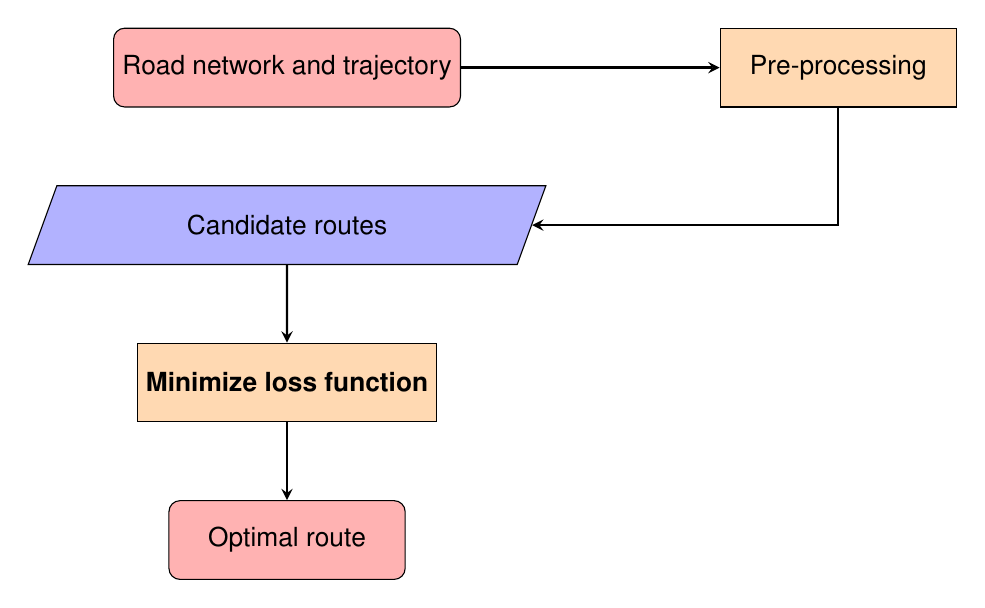
\begin{tikzpicture}[node distance=2cm]
\node (in1) [startstop] {Road network and trajectory};
\node (pre) [process, right of=in1, xshift=5cm] {Pre-processing};
%\node (pro1) [process, below of=in1] {Pre-processing};
\node (out1) [io, below of=in1] {Candidate routes};    
\node (pro2a) [process, below of=out1] {\textbf{Minimize loss function} };
\node (out2) [startstop, below of=pro2a] {Optimal route};


\draw [arrow] (in1) -- (pre);
\draw [arrow] (pre) |- (out1);
%\draw [arrow] (pro1) -- (out1);
\draw [arrow] (out1) -- (pro2a);
\draw [arrow] (pro2a) -- (out2);
\end{tikzpicture}}
\end{center}
\end{frame}







% \begin{frame}{Proof of Theorem $1^*$}
% \begin{multicols}{2}
% Suppose we have a network with \textbf{bounded branching}: networks such that each vertex has no more than two edges originating from it.
% \vspace{-1.5cm}
% \small{
% \begin{align*}
%     A &= (0,0,0)  \\
%     B &= (4\sqrt{n},0,0) \\
%     C &= (4\sqrt{n},2\sqrt{n},0)\\
%     D &= (0,2\sqrt{n},0)\\
%     A' &=(0,0,8\sqrt{n}) \\
%     B' &=  (4\sqrt{n},0,8\sqrt{n})\\
%     C' &= (4\sqrt{n},2\sqrt{n},8\sqrt{n})\\
%     D' &= (0,2\sqrt{n},8\sqrt{n}))
% \end{align*}}
% \includegraphics[scale=.425]{Parallelol.png}
% \end{multicols}
% \end{frame}



%%%%%%%%%%%%%%%%%%%%%%%%%%%%%%%%%%%%%%%%%%%%%%%%%%%%%%%%%%%%%%%%%%%%%
%%%%%%%%%%%%%%%%%%%%%%%%%%%%%%%%Final%%%%%%%%%%%%%%%%%%%%%%%%%%%%%%%%
%%%%%%%%%%%%%%%%%%%%%%%%%%%%%%%%%%%%%%%%%%%%%%%%%%%%%%%%%%%%%%%%%%%%%

%\section{Mathematical formulation}

% \begin{frame}{Mathematical formulation}
% \begin{small}
% \vspace{-2mm}
% \begin{definition}[Local Road Network Graph]
% \begin{itemize} \vspace{-1mm}
% \item \textbf{``local" road network graph:}\,
% A local area where we cannot determine the superiority or inferiority of candidate routes.
% %We will also denote the local road network graph as $G=(V,E)$ to simplify the symbols. 
% \vspace{-2mm}
% \item For the local road network graph as $G=(V,E)$, we define 
% \begin{align*}
%     \CR_G = \CR \:= \{ \text{all candidate routes for local road network graph} G\},
% \end{align*}
% where note that each $A\in\CR$ is the edge subset of (original) road network graph. \vspace{-2mm}
% \item The local road network graph $G=(V,E)\;(\subset\R^N)$ consists of the following:
% \begin{itemize} \vspace{-2mm}
%     \item[$\diamond$] $\dis E = \bigcup_{\text{route }A\in\CR} \{e_A \;|\; e_A\in\text{route }A\}$,
%     \item[$\diamond$] $V = \{ v\in\R^N\;|\; \text{there exist }e_1,e_2\in E \text{ such that } v\in e_1\cap e_2 \}$.
% \end{itemize} 
% \item Set $\ee$ as the unit vector parallel to $e$ for each $e\in E$.
%       Although there is a $180^\circ$ degree of freedom in the direction of $\ee$, either is fine for practical purposes.
% \end{itemize}
% \end{definition}
% \end{small}
% \end{frame}

\subsection{Mathematical assumption}

\begin{frame}{Mathematical Formulation}
\begin{small}
\vspace{-2mm}
\begin{columns}[t]
\begin{column}{0.7\textwidth}
%\vspace{-20mm}
\begin{tcolorbox}[colframe=green,
colback=green!10!white,
colbacktitle=green!40!white,
coltitle=black, fonttitle=\bfseries]
\textbf{\underline{Assumption}}\,
\begin{itemize}
\item Give the \textbf{GPS error} as $\err:\mathbf{p}\to\R_{\ge0}$ and assume that the \emph{spherically-symmetric probability measure} $\gamma_p$ (e.g. \emph{Gaussian measure}) is given such that
$$
\supp\gamma_p=B\big(p;\err(p)\big)\:=\Big\{x\in\R^N\;\big|\;d_{\R^N}(x,p)\leq\err(p)\Big\}.
$$
We assume that $p\in\mathbf{p}$ is truly located at $x$ with probability $\gamma_p(x)$. 
\item Suppose that \textbf{there is NO error with respect to the speed and direction information}.
\end{itemize}
\end{tcolorbox}
\end{column}
\begin{column}{0.3\textwidth} 
\vspace{1mm}
\centering
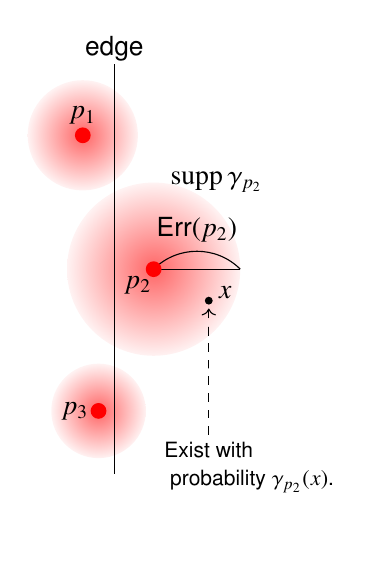
\begin{tikzpicture} %[every node/.style={circle,fill=white}]
\node (v1) at (0,3.2) {\text{edge}};
\shade[inner color=red!60!white, outer color=red!5!white] (-0.4,2.1) circle (0.7);
\shade[inner color=red!60!white, outer color=red!5!white] (0.5,0.4) circle (1.1);
\shade[inner color=red!60!white, outer color=red!5!white] (-0.2,-1.4) circle (0.6);
\draw[black] (0.5,0.4)--(1.6,0.4);
\path[draw] ($(0.5,0.4)$) 
to[out=45,in=135] ($(1.6,0.4)$);
\node (text) at (-0.4,2.35) {$p_1$};
\node (text) at (0.3,0.2) {$p_2$};
\node (text) at (-0.5,-1.4) {$p_3$};
\node (text) at (1.05,0.9) {$\err(p_2)$};
\node (text) at (1.3,1.5) {$\supp\gamma_{p_2}$};
\draw[black] (0,3)--(0,-2.2);
\fill[red] (-0.4,2.1) circle(0.1);
\fill[red] (0.5,0.4) circle(0.1);
\fill[red] (-0.2,-1.4) circle(0.1);
\fill[black] (1.2,0) circle(0.05);
\path[arrows=->, draw, dashed] ($(1.2,-1.7)$) 
to[out=90,in=270] ($(1.2,-0.1)$);
\node (p) at (1.4,0.1) {$x$};
\node (p) at (1.2,-1.9) {{\footnotesize Exist with }};
\node (p) at (1.75,-2.3) {{\footnotesize probability $\gamma_{p_2}(x)$.}};
\node (p) at (0,-3) {};
\end{tikzpicture}
\end{column}
\end{columns}
\end{small}
\end{frame}

\subsection{The ``distance" with error}

\begin{frame}
\begin{small}
\begin{definition}[The ``distance" with error between $p\in\mathbf{p}$ and $e\in E$] 
\bu Define the \textbf{``distance" with error} $\derr$ between $\cha(p)\in\mathbf{p}$ (\emph{\cha(with errors)}) and $e\in E$ (\emph{without errors}) as \vspace{-2mm}
\begin{align*}
    \derr(\cha(p),e) \:=  \int_{\cha(x_p)\in B\big(\cha(p);\err(p)\big)} d_{\R^N}(\cha(x_p),e)\, \dd\gamma_p(\cha(x_p)).
\end{align*}
\end{definition}
\centering
%\vspace{1mm}
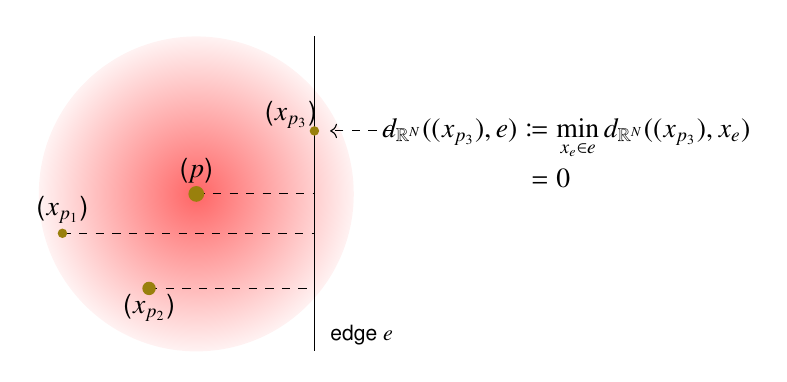
\begin{tikzpicture} %[every node/.style={circle,fill=white}]
\node (v) at (4,0) {};
\shade[inner color=red!60!white, outer color=red!5!white] (1.5,-2) circle (2);
\path[draw, thin, dashed] (1.5,-2)--(3,-2);
\path[draw, thin, dashed] (-0.2,-2.5)--(3,-2.5);
\path[draw, thin, dashed] (0.9,-3.2)--(3,-3.2);
\path[draw, ultra thin] (3,0)--(3,-4);
\node (p) at (1.5,-1.7) {\cha($p$)};
\node (p) at (-0.2,-2.2) {\cha($x_{p_1}$)};
\node (p) at (0.9,-3.45) {\cha($x_{p_2}$)};
\node (p) at (2.7,-1) {\cha($x_{p_3}$)};
\node (v1) at (3.6,-3.8) {{\footnotesize \text{edge }$e$}};
\path[arrows=->, draw, dashed] ($(4,-1.2)$) to[out=180,in=0] ($(3.2,-1.2)$);
\fill[DarkOrange] (1.5,-2) circle(0.1);
\fill[DarkOrange] (-0.2,-2.5) circle(0.06);
\fill[DarkOrange] (0.9,-3.2) circle(0.085);
\fill[DarkOrange] (3,-1.2) circle(0.06);
\node (p) at (6.2,-1.3) {$\dis d_{\R^N}(\cha(x_{p_3}),e) \:= \min_{x_e\in e} d_{\R^N}(\cha(x_{p_3}),x_e)$};
\node (p) at (6,-1.8) {$=0$};
\end{tikzpicture}
\begin{footnotesize}
\vspace{-7mm}
\begin{align*}
\end{align*}
\end{footnotesize}
\end{small}
\end{frame}


\section{Wasserstein method}

\subsection{Review of mid-term presentation}

\begin{frame}{Wasserstein method}
\begin{small}
\vspace{-1mm}
\begin{definition}[($L^1$-)Wasserstein distance (\emph{review of mid-term presentation})]
Let $(X,d)$ be a complete and separable metric space.
For probability measures $\mu,\nu$ \red(with finite supports), we define \emph{$W_1$ distance} between $\mu$ and $\nu$ as \vspace{-1.5mm}
$$
    W_1(\mu,\nu)\:=\min_{\pi\in\Pi(\mu,\nu)} \sum_{x\in X}\sum_{y\in X} d(x,y)\pi(x,y),
$$
where $\pi\in\Pi(\mu,\nu)$ $\;:\Leftrightarrow\;$ for any $x,y\in X$,\; $\sum_{y\in X}\pi(x,y)=\mu(x),\;\sum_{x\in X}\pi(x,y)=\nu(y)$. 
%\end{tcolorbox}
\end{definition}
\vspace{-2mm}
\begin{columns}[t]
\begin{column}{0.6\textwidth}
\vspace{-3mm}
\begin{definition}[Prob. meas. associated w/ $\mathbf{p}$ and $A\in\CR$]
\bu For the trajectory $\mathbf{p}$, define $\mu_\mathbf{p}\:=(1/n)\sum_{p\in\mathbf{p}}\delta_p$. \\
\bu $\triangleright$ Devide each $A\in\CR$ into $m+1$ equal parts and \\
\hspace{4.5mm} $V(A,m)$ denotes the set of $m$ threshold points. \\
\;\; $\triangleright$ Define $\nu_A\:=(1/m)\sum_{a\in V(A,m)}\delta_a$.
\end{definition}
\end{column}
\begin{column}{0.4\textwidth} 
\vspace{-9mm}
\begin{figure}[H]
\begin{tabular}{ccc}
\begin{minipage}{0.43\hsize}
\begin{center}
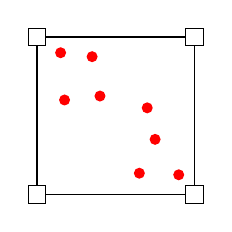
\begin{tikzpicture} %[every node/.style={circle,fill=white}]
\fill [red] (0.3,1.8) circle (0.07);
\fill [red] (0.7,1.75) circle (0.07);
\fill [red] (0.35,1.2) circle (0.07);
\fill [red] (0.8,1.25) circle (0.07);
\fill [red] (1.5,0.7) circle (0.07);
\fill [red] (1.4,1.1) circle (0.07);
\fill [red] (1.3,0.27) circle (0.07);
\fill [red] (1.8,0.25) circle (0.07);
\draw (0,2) node (v1) [draw] {};
\draw (2,2) node (v2) [draw] {};
\draw (0,0) node (v3) [draw] {};
\draw (2,0) node (v4) [draw] {};
\draw (v1)--(v2);
\draw (v2)--(v4);
\draw (v4)--(v3);
\draw (v3)--(v1);
\end{tikzpicture}
\end{center}
\end{minipage}
%%%%%%%%%%%%%%%%%%%%%%%%%%%%%%%%%%%%%%%%%%%%%%%%%%%%%%%%%%%%%%%%%%%%%%%%%%%%%%%%%%%%%%%%%%%%%%%%%%%%%%%%%%%%%%%%%%%%%%%%%%%%%%%%%%%%%%%%%%%%%%%%%%%%%%%%%%%%%%%%%%%%%%%
\begin{minipage}{0.1\hsize}
\begin{center}
\end{center}
\end{minipage}
%%%%%%%%%%%%%%%%%%%%%%%%%%%%%%%%%%%%%%%%%%%%%%%%%%%%%%%%%%%%%%%%%%%%%%%%%%%%%%%%%%%%%%%%%%%%%%%%%%%%%%%%%%%%%%%%%%%%%%%%%%%%%%%%%%%%%%%%%%%%%%%%%%%%%%%%%%%%%%%%%%%%%%%
\begin{minipage}{0.43\hsize}
\begin{center}
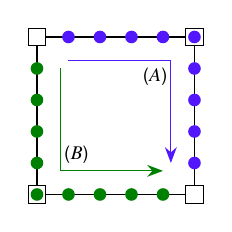
\begin{tikzpicture} %[every node/.style={circle,fill=white}]
\draw (0,2) node (v1) [draw] {};
\draw (2,2) node (v2) [draw] {};
\draw (0,0) node (v3) [draw] {};
\draw (2,0) node (v4) [draw] {};
\draw (v1)--(v2);
\draw (v2)--(v4);
\draw (v4)--(v3);
\draw (v3)--(v1);
\path[-{Stealth[length=2mm]}, draw=officegreen] ($(0.3,1.6)$) 
to[out=270,in=90] ($(0.3,0.3)$)
to[out=0,in=180] ($(1.6,0.3)$);
\path[-{Stealth[length=2mm]}, draw=hanpurple] ($(0.4,1.7)$) 
to[out=0,in=180] ($(1.7,1.7)$)
to[out=270,in=90] ($(1.7,0.4)$);
\node (x) at (1.5,1.5) {\scriptsize{\hanpurple($A$)}};
\node (x) at (0.5,0.5) {\scriptsize{\green($B$)}};
\fill [hanpurple] (0.4,2) circle (0.08);
\fill [hanpurple] (0.8,2) circle (0.08);
\fill [hanpurple] (1.2,2) circle (0.08);
\fill [hanpurple] (1.6,2) circle (0.08);
\fill [hanpurple] (2,2) circle (0.08);
\fill [hanpurple] (2,1.6) circle (0.08);
\fill [hanpurple] (2,1.2) circle (0.08);
\fill [hanpurple] (2,0.8) circle (0.08);
\fill [hanpurple] (2,0.4) circle (0.08);
\fill [officegreen] (0,1.6) circle (0.08);
\fill [officegreen] (0,1.2) circle (0.08);
\fill [officegreen] (0,0.8) circle (0.08);
\fill [officegreen] (0,0.4) circle (0.08);
\fill [officegreen] (0,0) circle (0.08);
\fill [officegreen] (0.4,0) circle (0.08);
\fill [officegreen] (0.8,0) circle (0.08);
\fill [officegreen] (1.2,0) circle (0.08);
\fill [officegreen] (1.6,0) circle (0.08);
\end{tikzpicture}
\end{center}
\end{minipage}
\end{tabular}
\end{figure} 
\vspace{-2mm} 
\hspace{-2.5mm} Compare $W_1(\mu_{\red(\mathbf{p})},\nu_{\blue(A)})$ with $W_1(\mu_{\red(\mathbf{p})},\nu_{\green(B)})$.
\end{column}
\end{columns}
\end{small}
\end{frame}




\begin{frame}{Wasserstein Distance: Proof of Concept}

\begin{figure}
\raggedleft
 \includegraphics[scale=.55]{Wass.png}
    %\caption{Caption}
    \label{wassTest}
\end{figure}
\end{frame}

\subsection{Motivation}

\begin{frame}{Motivation}
\begin{columns}[t]
\begin{column}{0.4\textwidth}
\vspace{-5mm}
\begin{figure}[H]
\begin{center}
\begin{tikzpicture} 
\draw (0,4) node (v1) [draw] {};
\draw (4,4) node (v2) [draw] {};
\draw (0,0) node (v3) [draw] {};
\draw (4,0) node (v4) [draw] {};
\draw (v1)--(v2);
\draw (v2)--(v4);
\draw (v4)--(v3);
\draw (v3)--(v1);
\uncover<2->{\path[-{Stealth[length=2mm]}, thick, draw] ($(2,3.5)$)--($(2,3.1)$);
\path[-{Stealth[length=2mm]}, thick, draw] ($(2,3)$)--($(2,2.6)$);
\path[-{Stealth[length=2mm]}, thick, draw] ($(2,2.5)$)--($(2,2.1)$);
\path[-{Stealth[length=2mm]}, thick, draw] ($(2.5,2)$)--($(2.9,2)$);
\path[-{Stealth[length=2mm]}, thick, draw] ($(3,2)$)--($(3.4,2)$);
\path[-{Stealth[length=2mm]}, thick, draw] ($(3.5,2)$)--($(3.9,2)$);}
\fill [red] (2,3.5) circle (0.07);
\fill [red] (2,3) circle (0.07);
\fill [red] (2,2.5) circle (0.07);
\fill [red] (2.5,2) circle (0.07);
\fill [red] (3,2) circle (0.07);
\fill [red] (3.5,2) circle (0.07);
\only<1-5>{\path[-{Stealth[length=2mm]}, draw=officegreen, dashed] ($(0.2,3.6)$) 
to[out=270,in=90] ($(0.2,0.2)$)
to[out=0,in=180] ($(3.6,0.2)$);}
\only<6>{\path[-{Stealth[length=4mm]}, draw=officegreen, ultra thick] ($(0.2,3.6)$) 
to[out=270,in=90] ($(0.2,0.2)$)
to[out=0,in=180] ($(3.6,0.2)$);}
\path[-{Stealth[length=2mm]}, draw=hanpurple, dashed] ($(0.4,3.8)$) 
to[out=0,in=180] ($(3.8,3.8)$)
to[out=270,in=90] ($(3.8,0.4)$);
\only<1>{\path[-{Stealth[length=4mm]}, draw=hanpurple, ultra thick] ($(0.4,3.8)$) 
to[out=0,in=180] ($(3.8,3.8)$)
to[out=270,in=90] ($(3.8,0.4)$);}
\node (x) at (3.5,3.5) {\hanpurple($A$)};
\node (x) at (0.5,0.5) {\green($B$)};
\end{tikzpicture}
\end{center}
\end{figure}
\vspace{-3mm}
\begin{small}
\bu Each $p\in\mathbf{p}$ is located on the \\ 
\hspace{3mm}vertical or parallel bisectors. \\
\uncover<2->{\bu $\spd(p)$, $\err(p)$ are the same at \\
\hspace{3mm}each $p$, respectively.}
\end{small}
\end{column}
\begin{column}{0.6\textwidth}
\vspace{-5mm}
\begin{small}
\begin{itemize}
\item Location only. \vspace{-1mm}
\item[$\triangleright$] $W_1(\mu_\mathbf{p},\nu_A)<W_1(\mu_\mathbf{p},\nu_B)$. %\vspace{1mm}
\uncover<2->{\item \textbf{We should select the route $B$}.} %\vspace{1mm}
\uncover<3->{\item Introduce probability measures $\mu_{\mathbf{p},A}^\eps$, $\nu_A^\eps$ and $\nu_B^\eps$ 
that include speed and direction information. \vspace{-1mm}
\item[$\triangleright$] Compare $W_1(\mu_{\mathbf{p},A}^\eps,\nu_A^\eps)$ with $W_1(\mu_{\mathbf{p},B}^\eps,\nu_B^\eps)$.} %\vspace{1mm}
\uncover<4->{\item[$\triangleright$] The effect of location is still strong.} %\vspace{1mm}
\uncover<5->{\item Normalization.} %\vspace{-1mm}
\only<5>{\item[$\triangleright$] Compare $\dis \frac{W_1(\mu_{\mathbf{p},A}^\eps,\nu_A^\eps)}{W_1(\mu_\mathbf{p},\nu_A)}$ 
with $\dis \frac{W_1(\mu_{\mathbf{p},B}^\eps,\nu_B^\eps)}{W_1(\mu_\mathbf{p},\nu_B)}$.} 
\only<6>{\item[$\triangleright$] $\dis \frac{W_1(\mu_{\mathbf{p},A}^\eps,\nu_A^\eps)}{W_1(\mu_\mathbf{p},\nu_A)} > \frac{W_1(\mu_{\mathbf{p},B}^\eps,\nu_B^\eps)}{W_1(\mu_\mathbf{p},\nu_B)}$.
\item[$\triangleright$] \textbf{We can select the route $B$.}}
\end{itemize}
\end{small}
\end{column}
\end{columns}
\end{frame}

\subsection{Our strategy}

\begin{frame}
\begin{small}
\vspace{-2mm}
\begin{tcolorbox}[colframe=yellow,
colback=yellow!10!white,
colbacktitle=yellow!40!white,
coltitle=black, fonttitle=\bfseries]
%\vspace{-2mm}
\textbf{\underline{Our strategy:}}\, 
Perturb $\mu_\mathbf{p}$ and each $\nu$ only by $\eps$ according to speed and direction. %\vspace{-1mm}
\end{tcolorbox}
\vspace{-1mm}
\bu Let $0<\eps\ll1$.
For each $p\in\mathbf{p}$, $A\in\CR$, $a\in V(A,m)$ and $x\in V(A,m)$, define \vspace{-2mm}

\only<1>{\[ \mu_{\mathbf{p},A}^\eps(x) \:= 
\begin{cases}
(1-\eps)/n & (x=p),   \\
\eps\cdot\big(\textbf{\red(our weight including $S\&D$)}\big) & (x\in V(A,m)), 
\end{cases}\]}
\only<2>{\[ \nu_A^\eps(x) \:= 
\begin{cases}
(1-\eps)/m & (x\in V(A,m)),   \\
\eps/n & (x\in\mathbf{p}).
\end{cases}\]}
%
\vspace{-8mm}
\only<1>{\begin{columns}[t]
\begin{column}{0.5\textwidth}
\begin{center}
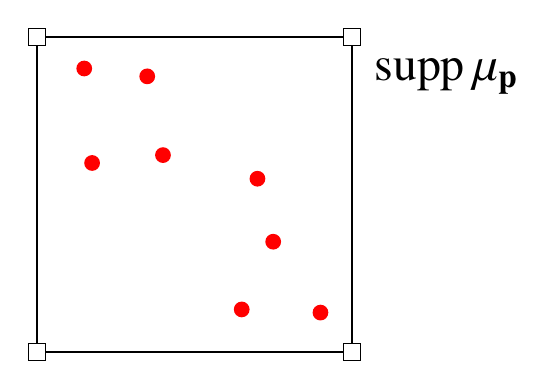
\begin{tikzpicture} %[every node/.style={circle,fill=white}]
\fill [red] (0.6,3.6) circle (0.1);
\fill [red] (1.4,3.5) circle (0.1);
\fill [red] (0.7,2.4) circle (0.1);
\fill [red] (1.6,2.5) circle (0.1);
\fill [red] (3,1.4) circle (0.1);
\fill [red] (2.8,2.2) circle (0.1);
\fill [red] (2.6,0.54) circle (0.1);
\fill [red] (3.6,0.5) circle (0.1);
\draw (0,4) node (v1) [draw] {};
\draw (4,4) node (v2) [draw] {};
\draw (0,0) node (v3) [draw] {};
\draw (4,0) node (v4) [draw] {};
\draw (v1)--(v2);
\draw (v2)--(v4);
\draw (v4)--(v3);
\draw (v3)--(v1);
\node (x) at (5.2,3.5) {{\LARGE $\supp\mu_\mathbf{p}$}};
\end{tikzpicture}
\end{center}
\end{column}
\begin{column}{0.5\textwidth} 
\begin{center}
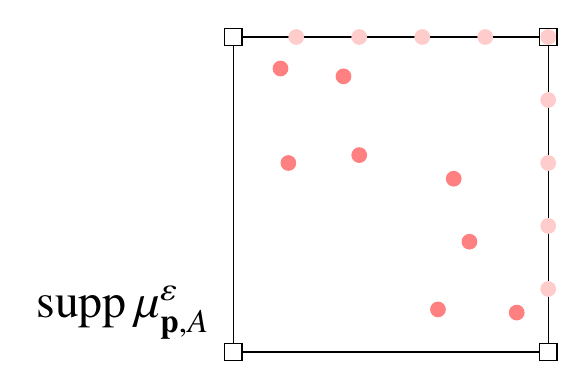
\begin{tikzpicture} %[every node/.style={circle,fill=white}]
\draw (0,4) node (v1) [draw] {};
\draw (4,4) node (v2) [draw] {};
\draw (0,0) node (v3) [draw] {};
\draw (4,0) node (v4) [draw] {};
\draw (v1)--(v2);
\draw (v2)--(v4);
\draw (v4)--(v3);
\draw (v3)--(v1);
\fill [red!50] (0.6,3.6) circle (0.1);
\fill [red!50] (1.4,3.5) circle (0.1);
\fill [red!50] (0.7,2.4) circle (0.1);
\fill [red!50] (1.6,2.5) circle (0.1);
\fill [red!50] (3,1.4) circle (0.1);
\fill [red!50] (2.8,2.2) circle (0.1);
\fill [red!50] (2.6,0.54) circle (0.1);
\fill [red!50] (3.6,0.5) circle (0.1);
%
\fill [red!20] (0.8,4) circle (0.1);
\fill [red!20] (1.6,4) circle (0.1);
\fill [red!20] (2.4,4) circle (0.1);
\fill [red!20] (3.2,4) circle (0.1);
\fill [red!20] (4,4) circle (0.1);
\fill [red!20] (4,3.2) circle (0.1);
\fill [red!20] (4,2.4) circle (0.1);
\fill [red!20] (4,1.6) circle (0.1);
\fill [red!20] (4,0.8) circle (0.1);
\node (x) at (-1.4,0.5) {{\LARGE $\supp\mu_{\mathbf{p},A}^\eps$}};
\end{tikzpicture}
\end{center}
\end{column}
\end{columns}}
%%%
\only<2>{\begin{columns}[t]
\begin{column}{0.5\textwidth}
\begin{center}
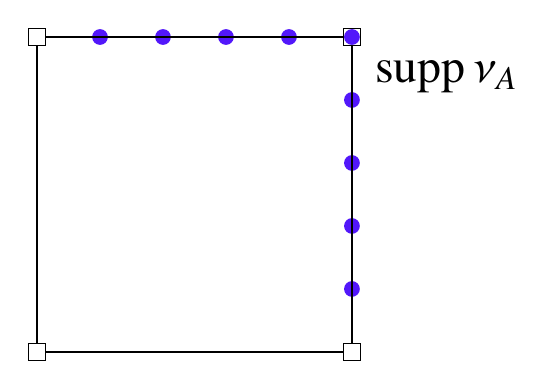
\begin{tikzpicture} %[every node/.style={circle,fill=white}]
\fill [hanpurple] (0.8,4) circle (0.1);
\fill [hanpurple] (1.6,4) circle (0.1);
\fill [hanpurple] (2.4,4) circle (0.1);
\fill [hanpurple] (3.2,4) circle (0.1);
\fill [hanpurple] (4,4) circle (0.1);
\fill [hanpurple] (4,3.2) circle (0.1);
\fill [hanpurple] (4,2.4) circle (0.1);
\fill [hanpurple] (4,1.6) circle (0.1);
\fill [hanpurple] (4,0.8) circle (0.1);
\draw (0,4) node (v1) [draw] {};
\draw (4,4) node (v2) [draw] {};
\draw (0,0) node (v3) [draw] {};
\draw (4,0) node (v4) [draw] {};
\draw (v1)--(v2);
\draw (v2)--(v4);
\draw (v4)--(v3);
\draw (v3)--(v1);
\node (x) at (5.2,3.5) {{\LARGE $\supp\nu_A$}};
\end{tikzpicture}
\end{center}
\end{column}
\begin{column}{0.5\textwidth} 
\begin{center}
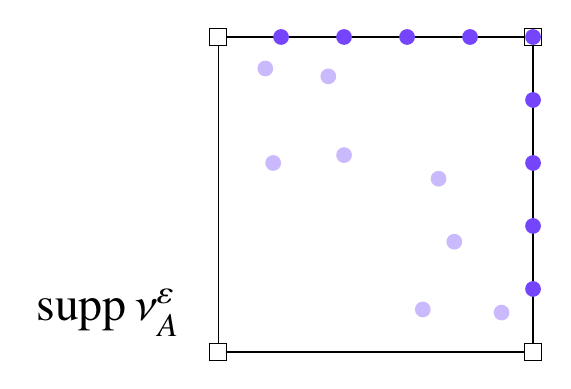
\begin{tikzpicture} %[every node/.style={circle,fill=white}]
\draw (0,4) node (v1) [draw] {};
\draw (4,4) node (v2) [draw] {};
\draw (0,0) node (v3) [draw] {};
\draw (4,0) node (v4) [draw] {};
\draw (v1)--(v2);
\draw (v2)--(v4);
\draw (v4)--(v3);
\draw (v3)--(v1);
\fill [hanpurple!30] (0.6,3.6) circle (0.1);
\fill [hanpurple!30] (1.4,3.5) circle (0.1);
\fill [hanpurple!30] (0.7,2.4) circle (0.1);
\fill [hanpurple!30] (1.6,2.5) circle (0.1);
\fill [hanpurple!30] (3,1.4) circle (0.1);
\fill [hanpurple!30] (2.8,2.2) circle (0.1);
\fill [hanpurple!30] (2.6,0.54) circle (0.1);
\fill [hanpurple!30] (3.6,0.5) circle (0.1);
%
\fill [hanpurple!80] (0.8,4) circle (0.1);
\fill [hanpurple!80] (1.6,4) circle (0.1);
\fill [hanpurple!80] (2.4,4) circle (0.1);
\fill [hanpurple!80] (3.2,4) circle (0.1);
\fill [hanpurple!80] (4,4) circle (0.1);
\fill [hanpurple!80] (4,3.2) circle (0.1);
\fill [hanpurple!80] (4,2.4) circle (0.1);
\fill [hanpurple!80] (4,1.6) circle (0.1);
\fill [hanpurple!80] (4,0.8) circle (0.1);
\node (x) at (-1.4,0.5) {{\LARGE $\supp\nu_A^\eps$}};
\end{tikzpicture}
\end{center}
\end{column}
\end{columns}}
\end{small}
\end{frame}

\subsection{Summary $\&$ Future problem}

\begin{frame}{Summary $\&$ Future problem}
\begin{small}
%\vspace{-2mm}
\begin{tcolorbox}[colframe=black,
colback=black!10!white,
colbacktitle=black!40!white,
coltitle=black, fonttitle=\bfseries]
\textbf{\underline{Summary}}\,
\begin{itemize}
\item Quantify the distance between $p\in\mathbf{p}$ and each $A\in\CR$ by making $\mu_\mathbf{p}$ and $\nu_A$ $\eps$-pertubation according to speed and direction information.
\item Conclude that \textbf{the route $A$ with the smallest $W_1(\mu_{\mathbf{p},A}^\eps,\nu_A^\eps)/W_1(\mu_\mathbf{p},\nu_A)$ is the true route}.
\end{itemize}
\end{tcolorbox}
\vspace{1mm}
\begin{tcolorbox}[colframe=yellow,
colback=yellow!10!white,
colbacktitle=yellow!40!white,
coltitle=black, fonttitle=\bfseries]
\textbf{\underline{Future problem (from a theoretical point of view)}}\,
\begin{itemize}
\item Is this method also effective when $\CR$ is dense?
\item Formulation of $\mu_\mathbf{p}$ with $(\gamma_p)_{p\in\mathbf{p}}$.
%\item Modification of the weight variance to the threshold points on each side according to the magnitude of speed.
%\item Is it possible to modify the $(\R^N)$-distance used for the $W_1$ distance with $\derr$?
\end{itemize}
\end{tcolorbox}
\end{small}
\end{frame}

%%%%%%%%%%%%%%%%%%%%%%%%%%%%%%%%%%%%%%%%%%%%%%%%%%%%%%%%%%%%%%%%%%%%%
%%%%%%%%%%%%%%%%%%%%%%%%%%%%%%%%Final%%%%%%%%%%%%%%%%%%%%%%%%%%%%%%%%
%%%%%%%%%%%%%%%%%%%%%%%%%%%%%%%%%%%%%%%%%%%%%%%%%%%%%%%%%%%%%%%%%%%%%







%%%%%%%%%%%%%%%%%%%%%%%%%%%%%%%%%%%%%%%%%%%%%%%%%%%%%%%%
%%%%%%%%%%%%%%%%%%%%%%%%%%%%%%%%%%%%%%%%%%%%%%%%%%%%%%%%
\section{``Physical'' method}

%%%%%%%%%%%%%%%%%%%%%%%%%%%%%%%%%%%%%%%%%%%%%%%%%%%%%%%%

\subsection{``Electric'' Method}

\begin{frame}{``Electric'' Method : Review of Mid-presentation}
\vspace{-5.5mm}
\begin{figure}[H]
\begin{tabular}{ccccc}
\begin{minipage}{0.25\hsize}
\begin{center}
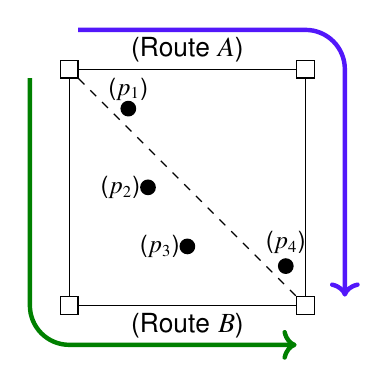
\begin{tikzpicture}
\node (p1) at (0.75,2.75) {{\small \red($p_{1}$)}};
\node (p2) at (0.65,1.5) {{\small \red($p_{2}$)}};
\node (p3) at (1.15,0.75) {{\small \red($p_{3}$)}};
\node (p4) at (2.75,0.8) {{\small \red($p_{4}$)}};
\draw (0,3) node (v1) [draw] {};%{$v_1$};
\draw (3,3) node (v2) [draw] {};%{$v_2$};
\draw (0,0) node (v3) [draw] {};%{$v_3$};
\draw (3,0) node (v4) [draw] {};%{$v_4$};
\draw (v1)--(v2);
\draw (v2)--(v4);
\draw (v4)--(v3);
\draw (v3)--(v1);
\draw[dashed] (v1)--(v4);
%\draw[red, dashed] (p3)--(pn-1);
%\draw[red, dashed] (p2)--(pn);
\node at (1.5,3.25) {{\hanpurple(Route $A$)}};
\path[arrows=->, ultra thick, draw=hanpurple] ($(v1)+(0.1125,0.5)$) 
to[out=0,in=180] ($(v2)+(0,0.5)$)
to[out=0,in=90] ($(v2)+(0.5,0)$)
to[out=270,in=90] ($(v4)+(0.5,0.1125)$);
\node at (1.5,-0.25) {{\green(Route $B$)}};
\path[arrows=->, ultra thick, draw=officegreen] ($(v1)+(-0.5,-0.1125)$) 
to[out=270,in=90] ($(v3)+(-0.5,0)$)
to[out=270,in=180] ($(v3)+(0,-0.5)$)
to[out=0,in=180] ($(v4)+(-0.1125,-0.5)$);
\fill (0.75,2.5) circle(0.1);
\fill (1,1.5) circle(0.1);
\fill (1.5,0.75) circle(0.1);
\fill (2.75,0.5) circle(0.1);
\end{tikzpicture}
\end{center}
\end{minipage}
%%%%%%%%%%%%%%%%%%%%%%%%%%%%
\begin{minipage}{0.1\hsize}
\begin{center}
\end{center}
\end{minipage}
%%%%%%%%%%%%%%%%%%%%%%%%%%%%
\begin{minipage}{0.25\hsize}
\begin{center}
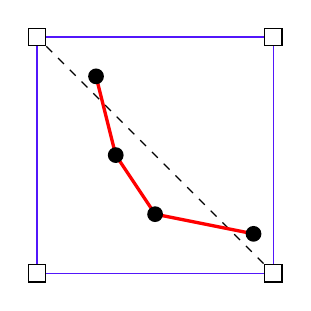
\begin{tikzpicture}%[every node/.style={circle,fill=white}]
\draw (0,3) node (v1) [draw] {};%{$v_1$};
\draw (3,3) node (v2) [draw] {};%{$v_2$};
\draw (0,0) node (v3) [draw] {};%{$v_3$};
\draw (3,0) node (v4) [draw] {};%{$v_4$};
%\node (x) at (1.5,3) {};
%\node (y) at (1.5,-0.5) {};
\draw[hanpurple] (v1)--(v2);
\draw[hanpurple] (v2)--(v4);
\draw[hanpurple] (v4)--(v3);
\draw[hanpurple] (v3)--(v1);
\draw[dashed] (v1)--(v4);
\draw[red, very thick] (0.75,2.5)--(1,1.5);
\draw[red, very thick] (1,1.5)--(1.5,0.75);
\draw[red, very thick] (1.5,0.75)--(2.75,0.5);
\fill (0.75,2.5) circle(0.1);
\fill (1,1.5) circle(0.1);
\fill (1.5,0.75) circle(0.1);
\fill (2.75,0.5) circle(0.1);
%\draw[red, dashed] (p1)--(pn-1);
%\draw[red, dashed] (p2)--(pn);
\end{tikzpicture}
%\vspace{-4mm}
\caption{{\footnotesize Connecting traj. pts. and giving charges.}}
\end{center}
\end{minipage}
%%%%%%%%%%%%%%%%%%%%%%%%%%%%
\begin{minipage}{0.1\hsize}
\begin{center}
\end{center}
\end{minipage}
%%%%%%%%%%%%%%%%%%%%%%%%%%%%
\begin{minipage}{0.25\hsize}
\begin{center}
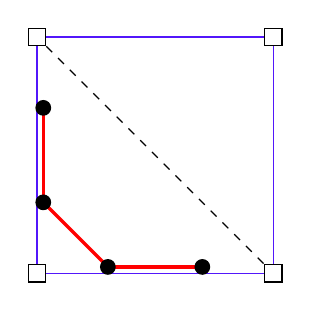
\begin{tikzpicture}%[every node/.style={circle,fill=white}]
\draw (0,3) node (v1) [draw] {};%{$v_1$};
\draw (3,3) node (v2) [draw] {};%{$v_2$};
\draw (0,0) node (v3) [draw] {};%{$v_3$};
\draw (3,0) node (v4) [draw] {};%{$v_4$};
\draw[hanpurple] (v1)--(v2);
\draw[hanpurple] (v2)--(v4);
\draw[hanpurple] (v4)--(v3);
\draw[hanpurple] (v3)--(v1);
\draw[dashed] (v1)--(v4);
\draw[red, very thick] (0.08,2.1)--(0.08,0.9);
\draw[red, very thick] (0.08,0.9)--(0.9,0.08);
\draw[red, very thick] (0.9,0.08)--(2.1,0.08);
\fill (0.08,2.1) circle(0.1);
\fill (0.08,0.9) circle(0.1);
\fill (0.9,0.08) circle(0.1);
\fill (2.1,0.08) circle(0.1);
\end{tikzpicture}
%\vspace{-4mm}
\caption{{\footnotesize Moving to ``closer'' route.}} 
\end{center}
\end{minipage}
\end{tabular}
\end{figure}
\begin{tcolorbox}[colframe=yellow,
colback=yellow!10!white,
colbacktitle=yellow!40!white,
coltitle=black, fonttitle=\bfseries]
\begin{itemize}
    \item
    Considering not only trajectory points, but also the entire polyline.  
\end{itemize}
%\textbf{Aim}: Comparing two entire routes rather than each edges. 
\end{tcolorbox}
%\hrulefill
\end{frame}



\begin{frame}{``Electric'' Method : Problems}
\vspace{-2mm}
\begin{tcolorbox}[colframe=yellow,
colback=yellow!10!white,
colbacktitle=yellow!40!white,
coltitle=black, fonttitle=\bfseries]
\vspace{-1mm}
\textbf{Problems}: 
    \begin{itemize}
        \item[\red($\times$)]
        Not taking into account speed and direction information.
        \item[\red($\times$)]
        Divergence problem : $\int_{\mathrm{polyline}}\int_{\mathrm{route}}r^{-2}$
        %\item[\red($\times$)]
        %Affects of crossing point is too large:
        \vspace{-2mm}
    \end{itemize}
\end{tcolorbox}
\vspace{-1mm}
\begin{itemize}
    \item
    Even if $\int_{\mathrm{polyline}}\int_{\mathrm{route}}(r^{2}+\varepsilon)^{-1}$, affects of intersection point is too large.
\end{itemize}
%%%%%%%%%%%%%%%%%%%%%%%%%%%%%
\vspace{-3.0mm}
\begin{figure}[H]
\begin{tabular}{ccccc}
\begin{minipage}{0.25\hsize}
%\vspace{-4mm}
\begin{center}
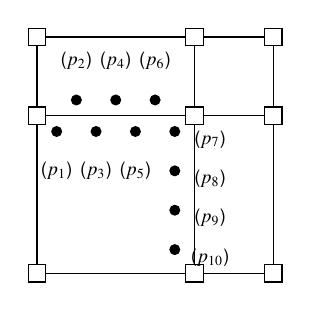
\begin{tikzpicture}%[every node/.style={circle,fill=white}]
      \fill (0.25,1.8) circle(0.07);
      \fill (0.5,2.2) circle(0.07);
      \fill (0.75,1.8) circle(0.07);
      \fill (1.0,2.2) circle(0.07);
      \fill (1.25,1.8) circle(0.07);
      \fill (1.5,2.2) circle(0.07);
      \fill (1.75,1.8) circle(0.07);
      \fill (1.75,1.3) circle(0.07);
      \fill (1.75,0.8) circle(0.07);
      \fill (1.75,0.3) circle(0.07);
      %%%%%%%%%%%%%%%%%%%%%%%%%%%%%%%%%%%%%%%
      \node (p1) at (0.25,1.3) {{\scriptsize \red($p_{1}$)}};
      \node (p2) at (0.5,2.7) {{\scriptsize \red($p_{2}$)}};
      \node (p3) at (0.75,1.3) {{\scriptsize \red($p_{3}$)}};
      \node (p4) at (1.0,2.7) {{\scriptsize \red($p_{4}$)}};
      \node (p5) at (1.25,1.3) {{\scriptsize \red($p_{5}$)}};
      \node (p6) at (1.5,2.7) {{\scriptsize \red($p_{6}$)}};
      \node (p7) at (2.2,1.7) {{\scriptsize \red($p_{7}$)}};
      \node (p8) at (2.2,1.2) {{\scriptsize \red($p_{8}$)}};
      \node (p9) at (2.2,0.7) {{\scriptsize \red($p_{9}$)}};
      \node (p10) at (2.2,0.2) {{\scriptsize \red($p_{10}$)}};
      %\fill (0.75,2.5) circle(0.1);
      %\fill (1,1.5) circle(0.1);
      %\fill (1.5,0.75) circle(0.1);  
      %\fill (2.75,0.5) circle(0.1);
      \draw (0,0) node (v1) [draw] {};
      \draw (2,0) node (v2) [draw] {};
      \draw (3,0) node (v3) [draw] {};
      \draw (0,2) node (v4) [draw] {};
      \draw (2,2) node (v5) [draw] {};
      \draw (3,2) node (v6) [draw] {};
      \draw (0,3) node (v7) [draw] {};
      \draw (2,3) node (v8) [draw] {};
      \draw (3,3) node (v9) [draw] {};
      \draw (v1)--(v2);
      \draw (v2)--(v3);
      \draw (v4)--(v5);
      \draw (v5)--(v6);
      \draw (v7)--(v8);
      \draw (v8)--(v9);
      \draw (v1)--(v4);
      \draw (v2)--(v5);
      \draw (v3)--(v6);
      \draw (v4)--(v7);
      \draw (v5)--(v8);
      \draw (v6)--(v9);
      \end{tikzpicture}
%\vspace{-4mm}

\end{center}
\end{minipage}
\begin{minipage}{0.1\hsize}
\begin{center}
\end{center}
\end{minipage}
%%%%%%%%%%%%%%%%%%%%%%%%%%%%
\begin{minipage}{0.25\hsize}
%\vspace{-4mm}
\begin{center}
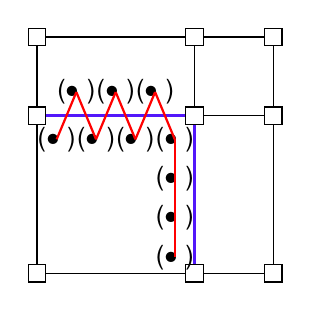
\begin{tikzpicture}%[every node/.style={circle,fill=white}]
      \node (p1) at (0.25,1.7) {\red(\bu)};
      \node (p2) at (0.5,2.3) {\red(\bu)};
      \node (p3) at (0.75,1.7) {\red(\bu)};
      \node (p4) at (1.0,2.3) {\red(\bu)};
      \node (p5) at (1.25,1.7) {\red(\bu)};
      \node (p6) at (1.5,2.3) {\red(\bu)};
      \node (p7) at (1.75,1.7) {\red(\bu)};
      \node (p8) at (1.75,1.2) {\red(\bu)};
      \node (p9) at (1.75,0.7) {\red(\bu)};
      \node (p10) at (1.75,0.2) {\red(\bu)};
      \draw (0,0) node (v1) [draw] {};
      \draw (2,0) node (v2) [draw] {};
      \draw (3,0) node (v3) [draw] {};
      \draw (0,2) node (v4) [draw] {};
      \draw (2,2) node (v5) [draw] {};
      \draw (3,2) node (v6) [draw] {};
      \draw (0,3) node (v7) [draw] {};
      \draw (2,3) node (v8) [draw] {};
      \draw (3,3) node (v9) [draw] {};
      %\draw (0,3) node (v1) [draw] {};
      %\draw (3,3) node (v2) [draw] {};
      %\draw (0,0) node (v3) [draw] {};
      %\draw (3,0) node (v4) [draw] {};
      \draw (v1)--(v2);
      \draw (v2)--(v3);
      \draw[hanpurple, very thick] (v4)--(v5);
      \draw (v5)--(v6);
      \draw (v7)--(v8);
      \draw (v8)--(v9);
      \draw (v1)--(v4);
      \draw[hanpurple, very thick] (v2)--(v5);
      \draw (v3)--(v6);
      \draw (v4)--(v7);
      \draw (v5)--(v8);
      \draw (v6)--(v9);
      \draw[red, thick](0.25,1.7)--(0.5,2.3);
      \draw[red, thick] (0.5,2.3)--(0.75,1.7);
      \draw[red, thick] (0.75,1.7)--(1.0,2.3);
      \draw[red, thick] (1.0,2.3)--(1.25,1.7);
      \draw[red, thick] (1.25,1.7)--(1.5,2.3);
      \draw[red, thick] (1.5,2.3)--(1.75,1.7);
      \draw[red, thick] (1.75,1.7)--(1.75,0.7);
      \draw[red, thick] (1.75,0.7)--(1.75,0.2);
      \end{tikzpicture}
%\vspace{-4mm}
\end{center}
\end{minipage}
%%%%%%%%%%%%%%%%%%%%%%%%%%%%
\begin{minipage}{0.1\hsize}
\begin{center}
\end{center}
\end{minipage}
%%%%%%%%%%%%%%%%%%%%%%%%%%%%
\begin{minipage}{0.25\hsize}
%\vspace{-4mm}
\begin{center}
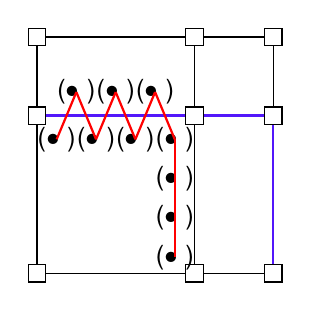
\begin{tikzpicture}%[every node/.style={circle,fill=white}]
      \node (p1) at (0.25,1.7) {\red(\bu)};
      \node (p2) at (0.5,2.3) {\red(\bu)};
      \node (p3) at (0.75,1.7) {\red(\bu)};
      \node (p4) at (1.0,2.3) {\red(\bu)};
      \node (p5) at (1.25,1.7) {\red(\bu)};
      \node (p6) at (1.5,2.3) {\red(\bu)};
      \node (p7) at (1.75,1.7) {\red(\bu)};
      \node (p8) at (1.75,1.2) {\red(\bu)};
      \node (p9) at (1.75,0.7) {\red(\bu)};
      \node (p10) at (1.75,0.2) {\red(\bu)};
      \draw (0,0) node (v1) [draw] {};
      \draw (2,0) node (v2) [draw] {};
      \draw (3,0) node (v3) [draw] {};
      \draw (0,2) node (v4) [draw] {};
      \draw (2,2) node (v5) [draw] {};
      \draw (3,2) node (v6) [draw] {};
      \draw (0,3) node (v7) [draw] {};
      \draw (2,3) node (v8) [draw] {};
      \draw (3,3) node (v9) [draw] {};
      %\draw (0,3) node (v1) [draw] {};
      %\draw (3,3) node (v2) [draw] {};
      %\draw (0,0) node (v3) [draw] {};
      %\draw (3,0) node (v4) [draw] {};
      \draw (v1)--(v2);
      \draw (v2)--(v3);
      \draw[hanpurple, very thick] (v4)--(v5);
      \draw[hanpurple, very thick] (v5)--(v6);
      \draw (v7)--(v8);
      \draw (v8)--(v9);
      \draw (v1)--(v4);
      \draw (v2)--(v5);
      \draw[hanpurple, thick] (v3)--(v6);
      \draw (v4)--(v7);
      \draw (v5)--(v8);
      \draw (v6)--(v9);
      \draw[red, thick](0.25,1.7)--(0.5,2.3);
      \draw[red, thick] (0.5,2.3)--(0.75,1.7);
      \draw[red, thick] (0.75,1.7)--(1.0,2.3);
      \draw[red, thick] (1.0,2.3)--(1.25,1.7);
      \draw[red, thick] (1.25,1.7)--(1.5,2.3);
      \draw[red, thick] (1.5,2.3)--(1.75,1.7);
      \draw[red, thick] (1.75,1.7)--(1.75,0.7);
      \draw[red, thick] (1.75,0.7)--(1.75,0.2);
      \end{tikzpicture}
%\vspace{-4mm}
\end{center}
\end{minipage}
\end{tabular}
\end{figure}
\end{frame}

\begin{frame}{``Electric'' Method : Strategy to Solve the Problems}
    \begin{tcolorbox}[colframe=yellow,
colback=yellow!10!white,
colbacktitle=yellow!40!white,
coltitle=black, fonttitle=\bfseries]
%\vspace{-1mm}
\textbf{Strategy}: 
    \begin{itemize}
        \item
        Replace ``maximizing inverse square'' to ``minimizing square'';
    \end{itemize}
    \begin{align*}
        \max_{A\in\CR} \frac{1}{r^{2}} : \text{``electric'' method}
    \end{align*}
    \begin{center}
    
\begin{tikzpicture}
    \draw[<-, black, very thick] (0,0)--(0,0.3);
    \end{tikzpicture}
    \end{center}
    \begin{align*}
        \min_{A\in\CR} r^{2} : \text{``harmonic oscillator'' method}
    \end{align*}
\end{tcolorbox}
\end{frame}


%%%%%%%%%%%%%%%%%%%%%%%%%%%%%%%%%%%%%%%%%%%%%%%%%%%%%%%%

\subsection{``Harmonic oscillator'' method}


\begin{frame}{``Harmonic Oscillator'' Method : General Setting}
\begin{columns}[t]
\begin{column}{0.5\textwidth}
\begin{small}
\vspace{-6mm}
\begin{center}
    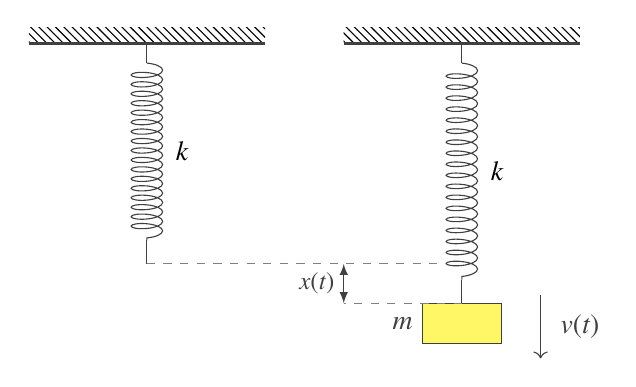
\begin{tikzpicture}[black!75]
		
		% Supporting structure
		\fill [pattern = north west lines] (-1.5,0) rectangle ++(3,.2);
		\draw[thick] (-1.5,0) -- ++(3,0);
		
		% Spring + Arrows
		\draw[] (0,0) -- ++(0,-0.25);
		\draw[decoration={aspect=0.3, segment length=1.2mm, amplitude=2mm,coil},decorate] (0,-0.25) -- ++(0,-2.25) node[midway,right=0.25cm,black]{$k$}; 
		\draw[] (0,-2.5) -- ++(0,-0.3) node[coordinate](c1){};
		
		\begin{scope}[xshift=4cm]
			% Supporting structure
			\fill [pattern = north west lines] (-1.5,0) rectangle ++(3,.2);
			\draw[thick] (-1.5,0) -- ++(3,0);
			
			% Spring + Arrows
			\draw[] (0,0) -- ++(0,-0.25);
			\draw[decoration={aspect=0.3, segment length=1.4mm, amplitude=2mm,coil},decorate] (0,-0.25) -- ++(0,-2.75) node[midway,right=0.25cm,black]{$k$}; 
			\draw[] (0,-3) -- ++(0,-0.3)node[coordinate](c2){} node[draw,fill=yellow!60,minimum width=1cm,minimum height=0.5cm,anchor=north,label=west:$m$](M){};
			\draw[<-] (1,-4)-- ++(0,0.8);
			\draw (1.5,-3.6) node (vt) {$v(t)$};
		\end{scope}
		
		\draw[dashed,gray] (c1) -- ++(3.75,0)coordinate(c22);
		\draw[dashed,gray] (c2) -- ++(-1.5,0) coordinate(c12);
		\draw[latex-latex] (c12)-- (c12|-c1)node[midway,left]{\small $x(t)$};
		
	\end{tikzpicture}
    \end{center}
\end{small}
\end{column}
\begin{column}{0.5\textwidth} 
\vspace{-3mm}
\begin{itemize}
    \item
    $m:$mass,
    \item
    $k:$spring constant,
    \item
    $v(t):$verocity of mass point,
    \item
    $x(t):$displacement from natural length of spring
    \item
    \emph{Lagrangian}
    \vspace{-3mm}
    \begin{align*}
        L(t) = \frac{1}{2}mv(t)^{2}+\frac{1}{2}kx(t)^{2}
    \end{align*}
    \item
    \emph{Action}
    \vspace{-3mm}
    \begin{align*}
        \mathsf{Act} = \int L(t)\,dt = \int\left\{\frac{1}{2}mv(t)^{2}+\frac{1}{2}kx(t)^{2}\right\}\,dt
    \end{align*}
\end{itemize}
\end{column}
\end{columns}
\end{frame}


\begin{frame}{``Harmonic Oscillator'' Method : Settings in Map-matching Problem}
\begin{columns}[t]
\begin{column}{0.5\textwidth}
\begin{small}
%\vspace{-3mm}
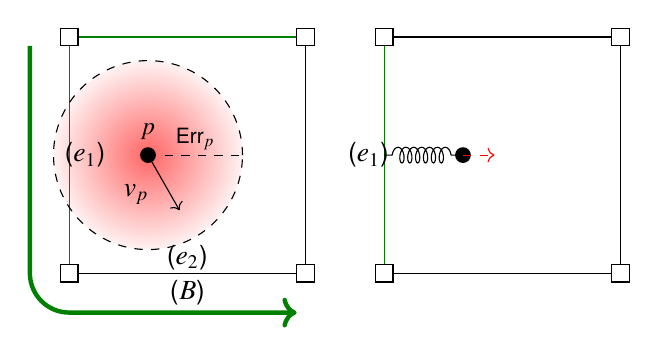
\begin{tikzpicture} 
\shade[inner color=red!60!white, outer color=red!5!white] (1,1.5) circle (1.2);
\node (p) at (1,1.8) {{\small $p$}};
\draw (0,3) node (v1) [draw] {};%{$v_1$};
\draw (3,3) node (v2) [draw] {};%{$v_2$};
\draw (0,0) node (v3) [draw] {};%{$v_3$};
\draw (3,0) node (v4) [draw] {};%{$v_4$};
\draw [officegreen] (v1)--(v2);
\draw (v2)--(v4);
\draw (v4)--(v3);
\draw [officegreen] (v3)--(v1);
\draw[->] (1,1.5) to (1.4,0.8);
%\draw[->, draw=red] (1,1.5) to (1.4,0.8);
\draw [dashed] (1,1.5) circle [radius=1.2];
\draw [dashed] (1,1.5) to (2.2,1.5);
\node (err) at (1.6,1.7)  {\footnotesize $\err_{p}$};
\node (e1) at (0.2,1.5) {\green($e_{1}$)};
\node (e2) at (1.5,0.2) {\green($e_{2}$)};
%\draw (1,1.5) to [dashed, out=90, in=90, edge node={node [midway,fill=white]{$\varepsilon$}}] (2.2,1.5);
%\fill [fill=black!10!white] (1,1.5) circle [radius=1.1];
\node (v) at (0.85,1.0) {$v_{p}$};%{\red($\spd$)};
\fill (1,1.5) circle(0.1);
\path[arrows=->, ultra thick, draw=officegreen] ($(v1)+(-0.5,-0.1125)$) 
to[out=270,in=90] ($(v3)+(-0.5,0)$)
to[out=270,in=180] ($(v3)+(0,-0.5)$)
to[out=0,in=180] ($(v4)+(-0.1125,-0.5)$);
\node at (1.5,-0.25) {\green($B$)};
    \begin{scope}[xshift=4cm]
%\node (p) at (1,1.8) {{\small \red($p$)}};
\draw (0,3) node (v1) [draw] {};%{$v_1$};
\draw (3,3) node (v2) [draw] {};%{$v_2$};
\draw (0,0) node (v3) [draw] {};%{$v_3$};
\draw (3,0) node (v4) [draw] {};%{$v_4$};
\draw (v1)--(v2);
\draw (v2)--(v4);
\draw (v4)--(v3);
\draw [officegreen] (v3)--(v1);
\node (e1) at (-0.2,1.5) {\green($e_{1}$)};
\draw
[
    decoration={
        coil,
        segment length = 1mm,
        amplitude = 1mm,
        aspect = 0.5,
        post length = 1mm,
        pre length = 1mm},
    decorate] (0,1.5) -- (1,1.5);
\fill (1,1.5) circle(0.1);
%\draw[->, draw=red] (1,1.5) to (1.4,0.8);
%\draw[dashed, ->, draw=red] (1,1.5) to (1,0.8);
\draw[dashed, ->, draw=red] (1,1.5) to (1.4,1.5);
%\draw (0,1.5) to [out=90, in=90, edge node={node [midway,fill=white]{$x$}}] (1,1.5);
%\node (v1) at (1.25,1.8) {$m$};
%\node (v1) at (1.9,1.5) {\red($\spd_{1}$)};
%\node (v2) at (0.5,1) {\red($\spd_{2}$)};
	\end{scope}
\end{tikzpicture}
\end{small}
\end{column}
\begin{column}{0.5\textwidth} 
\vspace{-3mm}
    \begin{itemize}
        \item
        $p\in\R^{N}$ : trajectory point,
        \item
        $v_{p}=\spd_{p}u_{p}\in\R^{N}$ : speed at $p$,
        \item
        $\err(p)\in\R$ : error of $p$,
        \item
        $B\in\CR, \quad e\in B$
        \vspace{3mm}
        \item
        $S(p,e) : \text{\emph{score} of edge $e$}$
    \end{itemize}
    \vspace{-3mm}
        \begin{align*}
            \:= \langle v,\vec{e}\rangle_{\R^{N}}\exp{\left(-\derr(p,e)\right)}%\quad(e:\mathrm{edge})
        \end{align*}
\end{column}
\end{columns}
\vspace{-4mm}
\begin{tcolorbox}[colframe=yellow,
colback=yellow!10!white,
colbacktitle=yellow!40!white,
coltitle=black, fonttitle=\bfseries]
    \begin{itemize}
        \item
        Connect trajectory point to the highest score edge by ``spring''.
        \item
        Define ``Lagrangian'' of this system.
    \end{itemize}
    %$\leadsto$ Defining 
\end{tcolorbox}
\end{frame}



\begin{frame}{``Harmonic Oscillator'' Method : Settings in Map-matching Problem}
\begin{columns}[t]
\begin{column}{0.3\textwidth}
\begin{small}
\begin{center}
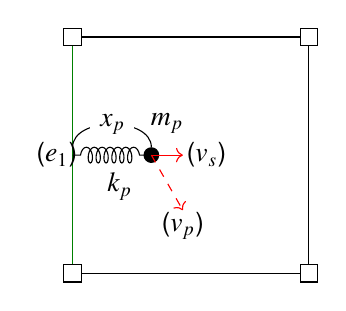
\begin{tikzpicture} 
%\node (p) at (1,1.8) {{\small \red($p$)}};
\draw (0,3) node (v1) [draw] {};%{$v_1$};
\draw (3,3) node (v2) [draw] {};%{$v_2$};
\draw (0,0) node (v3) [draw] {};%{$v_3$};
\draw (3,0) node (v4) [draw] {};%{$v_4$};
\draw (v1)--(v2);
\draw (v2)--(v4);
\draw (v4)--(v3);
\draw [officegreen] (v3)--(v1);
\node (e1) at (-0.2,1.5) {\green($e_{1}$)};
\draw
[
    decoration={
        coil,
        segment length = 1mm,
        amplitude = 1mm,
        aspect = 0.5,
        post length = 1mm,
        pre length = 1mm},
    decorate] (0,1.5) -- (1,1.5);
\fill (1,1.5) circle(0.1);
\draw[dashed, ->, draw=red] (1,1.5) to (1.4,0.8);
%\draw[dashed, ->, draw=red] (1,1.5) to (1,0.8);
\draw[->, draw=red] (1,1.5) to (1.4,1.5);
\draw (0,1.6) to [out=90, in=90, edge node={node [midway,fill=white]{$x_{p}$}}] (1,1.6);
\node (m) at (1.2,1.9) {$m_{p}$};
\node (k) at (0.6,1.1) {$k_{p}$};
\node (vs) at (1.7,1.5) {\red($v_{s}$)};
%\node (v2) at (0.5,1) {\red($v_{2}$)};
\node (v) at (1.4,0.6) {\red($v_{p}$)};
%\node (a) at (-0.3,1.5) {$a$};
\end{tikzpicture}
\end{center}
%\begin{itemize}
%    \item
%    $a$ : anchor of ``spring''. 
%\end{itemize}
%\vspace{-3mm}
\end{small}
\end{column}
\begin{column}{0.7\textwidth} 
%\vspace{-0.5cm}
    \begin{itemize}
        %\item
        %$\vec{s}$ : unit vector pointing  
        \item
        $v_{s}$ : spring direction component of $v_{p}$
        \item
        $x_{p}=d_{\err_{p}}(p,e)$ : ``displacement'' of $p$
        \item
        $m_{p} = \frac{1}{1+\err(p)}$ : ``mass'' of $p$,
        \item
        $k_{p} = \exp{\left(-\err(p)\right)}$ : ``spring constant'' w.r.t. $p$,
        \item
        $M(p) = m_{p}\left\|\frac{v_{s}}{\log(1+|v_{p}|)}\right\|^{2}$ : ``momentum'' of $p$,
        %= m_{p}\left\langle\frac{v_{s}}{\log(1+|v_{s}|)},p-a\right\rangle_{\R^{N}}^{2}$
        \item
        $P(p) = k_{p}x_{p}^{2}$ : ``potential'' of $p$,
    \end{itemize}
\end{column}
\end{columns}
\begin{tcolorbox}[colframe=yellow,
colback=yellow!10!white,
colbacktitle=yellow!40!white,
coltitle=black, fonttitle=\bfseries]
\vspace{-4mm}
    \begin{align*}
        L := M(p) + P(p) : \text{``Lagrangian''}.
    \end{align*}
    %$\leadsto$ Defining 
\end{tcolorbox}
\end{frame}


\begin{frame}{``Harmonic Oscillator'' Method : Settings in Map-matching Problem}
\begin{columns}[t]
\begin{column}{0.5\textwidth}
\vspace{-4mm}
\begin{small}
\begin{center}
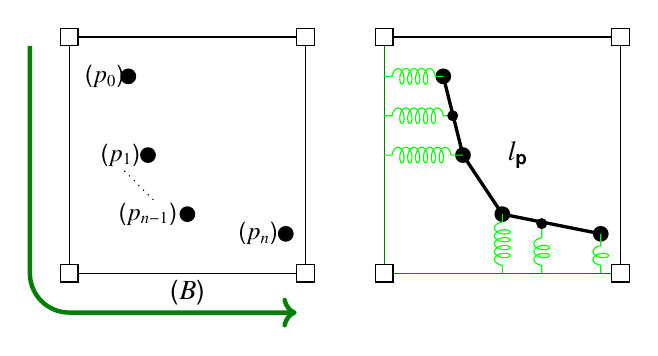
\begin{tikzpicture}%[every node/.style={circle,fill=white}]
\node (p0) at (0.45,2.5) {{\small \red($p_{0}$)}};
\node (p1) at (0.65,1.5) {{\small \red($p_{1}$)}};
\node (pn1) at (1,0.75) {{\small \red($p_{n-1}$)}};
\node (pn) at (2.4,0.5) {{\small \red($p_{n}$)}};
\draw (0,3) node (v1) [draw] {};%{$v_0$};
\draw (3,3) node (v2) [draw] {};%{$v_1$};
\draw (0,0) node (v3) [draw] {};%{$v_3$};
\draw (3,0) node (v4) [draw] {};%{$v_4$};
\draw (v1)--(v2);
\draw (v2)--(v4);
\draw (v4)--(v3);
\draw (v3)--(v1);
\draw [dotted] (0.7,1.3) to (1.1,0.9);
%\draw[dashed] (v1)--(v4);
\fill (0.75,2.5) circle(0.1);
\fill (1,1.5) circle(0.1);
\fill (1.5,0.75) circle(0.1);
\fill (2.75,0.5) circle(0.1);
\path[arrows=->, ultra thick, draw=officegreen] ($(v1)+(-0.5,-0.1125)$) 
to[out=270,in=90] ($(v3)+(-0.5,0)$)
to[out=270,in=180] ($(v3)+(0,-0.5)$)
to[out=0,in=180] ($(v4)+(-0.1125,-0.5)$);
\node at (1.5,-0.25) {\green($B$)};
    \begin{scope}[xshift=4cm]
\draw (0,3) node (v1) [draw] {};%{$v_1$};
\draw (3,3) node (v2) [draw] {};%{$v_2$};
\draw (0,0) node (v3) [draw] {};%{$v_3$};
\draw (3,0) node (v4) [draw] {};%{$v_4$};
%\node (x) at (1.5,3) {};
%\node (y) at (1.5,-0.5) {};
\draw (v1)--(v2);
\draw (v2)--(v4);
\draw [officegreen](v4)--(v3);
\draw [officegreen](v3)--(v1);
%\draw[hanpurple] (v1)--(v2);
%\draw[hanpurple] (v2)--(v4);
%\draw[hanpurple] (v4)--(v3);
%\draw[hanpurple] (v3)--(v1);
%\draw[dashed] (v1)--(v4);
\draw[very thick] (0.75,2.5)--(1,1.5);
\draw[very thick] (1,1.5)--(1.5,0.75);
\draw[very thick] (1.5,0.75)--(2.75,0.5);
\fill (0.75,2.5) circle(0.1);
\fill (1,1.5) circle(0.1);
\fill (1.5,0.75) circle(0.1);
\fill (2.75,0.5) circle(0.1);
%\draw[red, dashed] (p1)--(pn-1);
%\draw[red, dashed] (p2)--(pn);
\draw
[green,
    decoration={
        coil,
        segment length = 1mm,
        amplitude = 1mm,
        aspect = 0.5,
        post length = 1mm,
        pre length = 1mm},
    decorate] (0,2.5) -- (0.75,2.5);
%\fill (0.87,2) circle(0.07);
\draw
[green,
    decoration={
        coil,
        segment length = 1mm,
        amplitude = 1mm,
        aspect = 0.5,
        post length = 1mm,
        pre length = 1mm},
    decorate] (0,2) -- (0.9,2);
\fill (0.87,2) circle(0.07);
\draw
[green,
    decoration={
        coil,
        segment length = 1mm,
        amplitude = 1mm,
        aspect = 0.5,
        post length = 1mm,
        pre length = 1mm},
    decorate] (0,1.5) -- (1,1.5);
%\fill (0.87,2) circle(0.07);
\draw
[green,
    decoration={
        coil,
        segment length = 1mm,
        amplitude = 1mm,
        aspect = 0.5,
        post length = 1mm,
        pre length = 1mm},
    decorate] (1.5,0) -- (1.5,0.75);
%\fill (1.9,0.65) circle(0.07);
\draw
[green,
    decoration={
        coil,
        segment length = 1mm,
        amplitude = 1mm,
        aspect = 0.5,
        post length = 1mm,
        pre length = 1mm},
    decorate] (2,0) -- (2,0.63);
\fill (2,0.63) circle(0.07);
\draw
[green,
    decoration={
        coil,
        segment length = 1mm,
        amplitude = 1mm,
        aspect = 0.5,
        post length = 1mm,
        pre length = 1mm},
    decorate] (2.75,0) -- (2.75,0.5);
%\fill (1.9,0.65) circle(0.07);
\draw (1.7,1.5) node (lt) {$l_{\textbf{p}}$};
	\end{scope}
\end{tikzpicture}
%\vspace{-4mm}
%\caption{{\footnotesize Connecting traj. pts. and giving charges.}}
\end{center}
%\begin{itemize}
%    \item
%    $a$ : anchor of ``spring''. 
%\end{itemize}
%\vspace{-3mm}
\end{small}
\end{column}
\begin{column}{0.5\textwidth} 
\vspace{-3mm}
    \begin{itemize}
        \item
        $\mathbf{p} = (p_{i})_{0\le i\le n}$ : traj. points,
        \item
        $v_{\textbf{p}} = (v_{i}=\spd_{i}u_{i})_{0\le i\le n}$ : velocity,
        \item
        $\err:\textbf{p}\to\R$ : error,
        \item
        $B\in\CR$ : route.
    \end{itemize}
\vspace{-3mm}
\begin{center}
    
\begin{tikzpicture}
    \draw[<-, black, very thick] (0,0)--(0,0.3);
    \end{tikzpicture}
\end{center}
\vspace{-3mm}
\begin{itemize}
    \item
    $l_{\textbf{p}}:[0,1]\to\R^{N}$ : polyline,
    \item
    $v_{l_{\textbf{p}}}:[0,1]\to\R^{N}$ : velocity,
    \item
    $\err_{l_{\textbf{p}}}:[0,1]\to\R$ : error,
\end{itemize}
\end{column}
\end{columns}
\begin{tcolorbox}[colframe=yellow,
colback=yellow!10!white,
colbacktitle=yellow!40!white,
coltitle=black, fonttitle=\bfseries]
\vspace{-6.5mm}
    \begin{align*}
        L(t):=M(l_{\textbf{p}}(t))+P(l_{\textbf{p}}(t)),\quad Act_{\textbf{p}}(B) := \int_{[0,1]}\,L(t)\,dt : \text{``action'' of $\mathbf{p}$ on $B$}.
    \end{align*}
    %$\leadsto$ Defining 
    \vspace{-7mm}
\end{tcolorbox}
\end{frame}


\begin{frame}{``Harmonic Oscillator'' Method : Settings in Map-matching Problem}
\vspace{-5.5mm}
\begin{figure}[H]
\begin{tabular}{ccccc}
\begin{minipage}{0.25\hsize}
\begin{center}
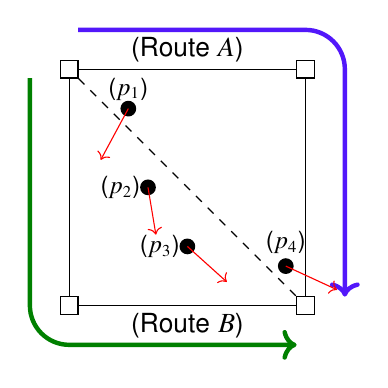
\begin{tikzpicture} 
%[every node/.style={circle,fill=white}] 
%\node (text1) at (-4,3.2) {\hspace{-52.5mm}\bu $V=\{v_1,v_2,v_3,v_4\}$,};
%\node (text2) at (-4,2.7) {\hspace{-35mm}$E=\{v_1v_2,v_2v_4,v_1v_3,v_3v_4\}$.};
%\node (text3) at (1.8,4.2) {\hspace{-8.3mm}\bu $\mathbf{p}=\{p_{1},p_{2},p_{3},p_{4}\}$};
%(-6.0,2.0)
%\node (text4) at (-4,1.0) {\hspace{-45.1mm}\bu \hanpurple(Route) $\hanpurple(\mathbf{A})=\{v_1v_2,v_2v_4\}$.};
%\node (text5) at (-4,0.5) {\hspace{-44.7mm}\bu \officegreen(Route) $\officegreen(\mathbf{B})=\{v_1v_3,v_3v_4\}$.};
\node (p1) at (0.75,2.75) {{\small \red($p_{1}$)}};
\node (p2) at (0.65,1.5) {{\small \red($p_{2}$)}};
\node (p3) at (1.15,0.75) {{\small \red($p_{3}$)}};
\node (p4) at (2.75,0.8) {{\small \red($p_{4}$)}};
\draw (0,3) node (v1) [draw] {};%{$v_1$};
\draw (3,3) node (v2) [draw] {};%{$v_2$};
\draw (0,0) node (v3) [draw] {};%{$v_3$};
\draw (3,0) node (v4) [draw] {};%{$v_4$};
\draw (v1)--(v2);
\draw (v2)--(v4);
\draw (v4)--(v3);
\draw (v3)--(v1);
\draw[dashed] (v1)--(v4);
%\draw[red, dashed] (p3)--(pn-1);
%\draw[red, dashed] (p2)--(pn);
\node at (1.5,3.25) {{\hanpurple(Route $A$)}};
\node at (1.5,-0.25) {{\green(Route $B$)}};
\path[arrows=->, ultra thick, draw=hanpurple] ($(v1)+(0.1125,0.5)$) 
to[out=0,in=180] ($(v2)+(0,0.5)$)
to[out=0,in=90] ($(v2)+(0.5,0)$)
to[out=270,in=90] ($(v4)+(0.5,0.1125)$);
\path[arrows=->, ultra thick, draw=officegreen] ($(v1)+(-0.5,-0.1125)$) 
to[out=270,in=90] ($(v3)+(-0.5,0)$)
to[out=270,in=180] ($(v3)+(0,-0.5)$)
to[out=0,in=180] ($(v4)+(-0.1125,-0.5)$);
\fill (0.75,2.5) circle(0.1);
\fill (1,1.5) circle(0.1);
\fill (1.5,0.75) circle(0.1);
\fill (2.75,0.5) circle(0.1);
\draw[->, draw=red] (0.75,2.5) to (0.4,1.85);
\draw[->, draw=red] (1,1.5) to (1.1,0.9);
\draw[->, draw=red] (1.5,0.75) to (2,0.3);
\draw[->, draw=red] (2.75,0.5) to (3.4,0.2);
\end{tikzpicture}
\end{center}
\end{minipage}
%%%%%%%%%%%%%%%%%%%%%%%%%%%%
\begin{minipage}{0.1\hsize}
\begin{center}
\end{center}
\end{minipage}
%%%%%%%%%%%%%%%%%%%%%%%%%%%%
\begin{minipage}{0.25\hsize}
\begin{center}
\vspace{2mm}
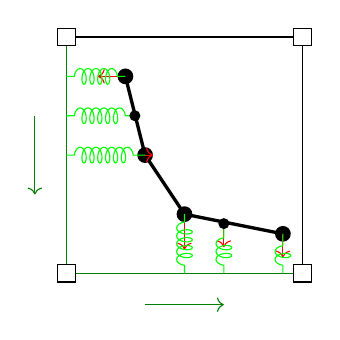
\begin{tikzpicture}%[every node/.style={circle,fill=white}]
\draw (0,3) node (v1) [draw] {};%{$v_1$};
\draw (3,3) node (v2) [draw] {};%{$v_2$};
\draw (0,0) node (v3) [draw] {};%{$v_3$};
\draw (3,0) node (v4) [draw] {};%{$v_4$};
%\node (x) at (1.5,3) {};
%\node (y) at (1.5,-0.5) {};
\draw (v1)--(v2);
\draw (v2)--(v4);
\draw[officegreen] (v4)--(v3);
\draw[officegreen] (v3)--(v1);
\draw[->, draw=officegreen] (-0.4,2) to (-0.4,1);
\draw[->, draw=officegreen] (1,-0.4) to (2,-0.4);
%\draw[dashed] (v1)--(v4);
\draw[very thick] (0.75,2.5)--(1,1.5);
\draw[very thick] (1,1.5)--(1.5,0.75);
\draw[very thick] (1.5,0.75)--(2.75,0.5);
\fill (0.75,2.5) circle(0.1);
\fill (1,1.5) circle(0.1);
\fill (1.5,0.75) circle(0.1);
\fill (2.75,0.5) circle(0.1);
\draw[->, draw=red] (0.75,2.5) to (0.4,2.5);
\draw[->, draw=red] (1,1.5) to (1.1,1.5);
\draw[->, draw=red] (1.5,0.75) to (1.5,0.3);
\draw[->, draw=red] (2,0.63) to (2,0.33);
\draw[->, draw=red] (2.75,0.5) to (2.75,0.2);
%\draw[red, dashed] (p1)--(pn-1);
%\draw[red, dashed] (p2)--(pn);
\draw
[green,
    decoration={
        coil,
        segment length = 1mm,
        amplitude = 1mm,
        aspect = 0.5,
        post length = 1mm,
        pre length = 1mm},
    decorate] (0,2.5) -- (0.75,2.5);
%\fill (0.87,2) circle(0.07);
\draw
[green,
    decoration={
        coil,
        segment length = 1mm,
        amplitude = 1mm,
        aspect = 0.5,
        post length = 1mm,
        pre length = 1mm},
    decorate] (0,2) -- (0.9,2);
\fill (0.87,2) circle(0.07);
\draw
[green,
    decoration={
        coil,
        segment length = 1mm,
        amplitude = 1mm,
        aspect = 0.5,
        post length = 1mm,
        pre length = 1mm},
    decorate] (0,1.5) -- (1,1.5);
%\fill (0.87,2) circle(0.07);
\draw
[green,
    decoration={
        coil,
        segment length = 1mm,
        amplitude = 1mm,
        aspect = 0.5,
        post length = 1mm,
        pre length = 1mm},
    decorate] (1.5,0) -- (1.5,0.75);
%\fill (1.9,0.65) circle(0.07);
\draw
[green,
    decoration={
        coil,
        segment length = 1mm,
        amplitude = 1mm,
        aspect = 0.5,
        post length = 1mm,
        pre length = 1mm},
    decorate] (2,0) -- (2,0.63);
\fill (2,0.63) circle(0.07);
\draw
[green,
    decoration={
        coil,
        segment length = 1mm,
        amplitude = 1mm,
        aspect = 0.5,
        post length = 1mm,
        pre length = 1mm},
    decorate] (2.75,0) -- (2.75,0.5);
\end{tikzpicture}
%\vspace{-4mm}
%\caption{{\footnotesize Connecting traj. pts. and giving charges.}}
\end{center}
\end{minipage}
%%%%%%%%%%%%%%%%%%%%%%%%%%%%
\begin{minipage}{0.1\hsize}
\begin{center}
\end{center}
\end{minipage}
%%%%%%%%%%%%%%%%%%%%%%%%%%%%
\begin{minipage}{0.25\hsize}
\begin{center}
\vspace{-4mm}
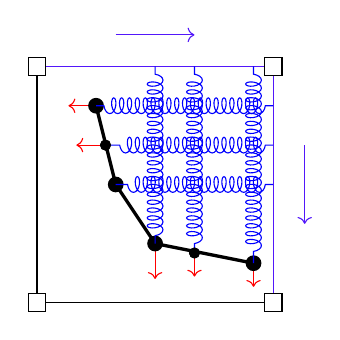
\begin{tikzpicture}%[every node/.style={circle,fill=white}]
\draw (0,3) node (v1) [draw] {};%{$v_1$};
\draw (3,3) node (v2) [draw] {};%{$v_2$};
\draw (0,0) node (v3) [draw] {};%{$v_3$};
\draw (3,0) node (v4) [draw] {};%{$v_4$};
%\node (x) at (1.5,3) {};
%\node (y) at (1.5,-0.5) {};
\draw[hanpurple] (v1)--(v2);
\draw[hanpurple] (v2)--(v4);
\draw (v4)--(v3);
\draw (v3)--(v1);
\draw[->, draw=hanpurple] (3.4,2) to (3.4,1);
\draw[->, draw=hanpurple] (1,3.4) to (2,3.4);
\draw[->, draw=red] (0.75,2.5) to (0.4,2.5);
\draw[->, draw=red] (0.87,2) to (0.5,2);
\draw[->, draw=red] (1,1.5) to (1.1,1.5);
\draw[->, draw=red] (1.5,0.75) to (1.5,0.3);
\draw[->, draw=red] (2,0.63) to (2,0.33);
\draw[->, draw=red] (2.75,0.5) to (2.75,0.2);
%\draw[dashed] (v1)--(v4);
\draw[very thick] (0.75,2.5)--(1,1.5);
\draw[very thick] (1,1.5)--(1.5,0.75);
\draw[very thick] (1.5,0.75)--(2.75,0.5);
\fill (0.75,2.5) circle(0.1);
\fill (1,1.5) circle(0.1);
\fill (1.5,0.75) circle(0.1);
\fill (2.75,0.5) circle(0.1);
\fill (0.87,2) circle(0.07);
\fill (2,0.63) circle(0.07);
%\draw[red, dashed] (p1)--(pn-1);
%\draw[red, dashed] (p2)--(pn);
\draw
[blue,
    decoration={
        coil,
        segment length = 1mm,
        amplitude = 1mm,
        aspect = 0.5,
        post length = 1mm,
        pre length = 1mm},
    decorate] (3,2.5) -- (0.75,2.5);
%\fill (0.87,2) circle(0.07);
\draw
[blue,
    decoration={
        coil,
        segment length = 1mm,
        amplitude = 1mm,
        aspect = 0.5,
        post length = 1mm,
        pre length = 1mm},
    decorate] (3,2) -- (0.9,2);
\fill (0.87,2) circle(0.07);
\draw
[blue,
    decoration={
        coil,
        segment length = 1mm,
        amplitude = 1mm,
        aspect = 0.5,
        post length = 1mm,
        pre length = 1mm},
    decorate] (3,1.5) -- (1,1.5);
%\fill (0.87,2) circle(0.07);
\draw
[blue,
    decoration={
        coil,
        segment length = 1mm,
        amplitude = 1mm,
        aspect = 0.5,
        post length = 1mm,
        pre length = 1mm},
    decorate] (1.5,3) -- (1.5,0.75);
%\fill (1.9,0.65) circle(0.07);
\draw
[blue,
    decoration={
        coil,
        segment length = 1mm,
        amplitude = 1mm,
        aspect = 0.5,
        post length = 1mm,
        pre length = 1mm},
    decorate] (2,3) -- (2,0.63);
\fill (2,0.63) circle(0.07);
\draw
[blue,
    decoration={
        coil,
        segment length = 1mm,
        amplitude = 1mm,
        aspect = 0.5,
        post length = 1mm,
        pre length = 1mm},
    decorate] (2.75,3) -- (2.75,0.5);
\end{tikzpicture}
%\vspace{-4mm}
%\caption{{\footnotesize Connecting traj. pts. and giving charges.}}
\end{center}
\end{minipage}
\end{tabular}
\end{figure}
\begin{tcolorbox}[colframe=yellow,
colback=yellow!10!white,
colbacktitle=yellow!40!white,
coltitle=black, fonttitle=\bfseries]
\begin{itemize}
    \item
    Calculate $Act_{\textbf{p}}(A)$ and $Act_{\textbf{p}}(B)$.
    \item
    Choose the route that minimize action.
\end{itemize}
\end{tcolorbox}
\end{frame}

\begin{frame}{``Harmonic Oscillator'' Method : Strength/Weakness and Future Problem}
    \begin{tcolorbox}[colframe=yellow,
    colback=yellow!10!white,
    colbacktitle=yellow!40!white,
    coltitle=black, fonttitle=\bfseries]
    \textbf{Strength/weakness}:
    \begin{itemize}
        \item[$\checkmark$]
        No divergence problem,
        \item[$\checkmark$]
        Taking into account speed and direction naturally,
        \item[\red($\times$)]
        Insufficient consideration of the entire route.
    \end{itemize}
    
    \textbf{Future problems}: 
    \begin{itemize}
        \item
        Consider more appropriate way to define mass and spring constant.
        \item
        Connect to all edge of a route with appropriate weight to consider the whole route.
    \end{itemize}
\end{tcolorbox}
\end{frame}

\begin{frame}{``Electric Method" and "Harmonic Oscillator": Proof of Concept}
    \begin{figure}
        \raggedleft
\includegraphics[scale=.55]{MaxNN.jpeg}
        %\caption{Caption}
        \label{Electrical Method with Maximum Nearest Neighbor}
    \end{figure}
\end{frame}

%%%%%%%%%%%%%%%%%%%%%%%%%%%%%%%%%%%%%%%%%%%%%%%%%%%%%%%%%%%%%%%%%
%%%%%%%%%%%%%%%%%%%%%%%%%%%%%%%%%%%%%%%%%%%%%%%%%%%%%%%%%%%%%%%%%

\section{Numerical Results}

\subsection{Implementation}

\begin{frame}{Implementing metric-based methods}
\vspace{-.1cm}
\centering
\includegraphics[scale=0.27]{Jupyter Notebook LaTeX/codeexample.png}

\end{frame}

\begin{frame}{Implementing metric-based methods}

Why are we defining each of the metric-based functions here, instead of in a separate Class? Because metric\_mm is designed to accommodate any distance-based loss function, allowing for simple and customizable simulator creations.

\centering
\includegraphics[scale=0.5]{Jupyter Notebook LaTeX/codeexample1.png}
\end{frame}

\subsection{Sendai Revisited}

\begin{frame}{Sendai Map Revisited}
Now we revisit the Sendai map case.
\end{frame}

\begin{frame}{Map-matching Pipeline}
\begin{center}
\scalebox{0.9}{
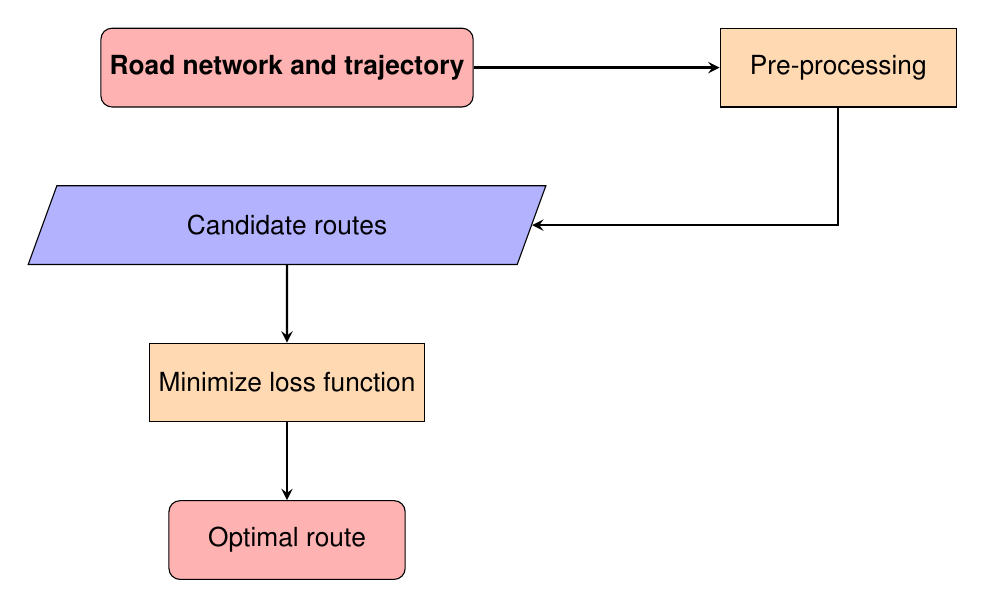
\begin{tikzpicture}[node distance=2cm]
\node (in1) [startstop] {\textbf{Road network and trajectory}};
\node (pre) [process, right of=in1, xshift=5cm] {Pre-processing};
%\node (pro1) [process, below of=in1] {Pre-processing};
\node (out1) [io, below of=in1] {Candidate routes};    
\node (pro2a) [process, below of=out1] {Minimize loss function };
\node (out2) [startstop, below of=pro2a] {Optimal route};


\draw [arrow] (in1) -- (pre);
\draw [arrow] (pre) |- (out1);
%\draw [arrow] (pro1) -- (out1);
\draw [arrow] (out1) -- (pro2a);
\draw [arrow] (pro2a) -- (out2);
\end{tikzpicture}}
\end{center}
\end{frame}



\begin{frame}{Sendai Map Revisited}
\vspace{-.1cm}
       \begin{figure}
        \centering
        \includegraphics[scale=.42]{trajectoryandroads.png}
   %     \caption{Caption}
   %     \label{fig:my_label}
    \end{figure} 
\end{frame}


\begin{frame}{Map-matching Pipeline}
\begin{center}
\scalebox{0.9}{
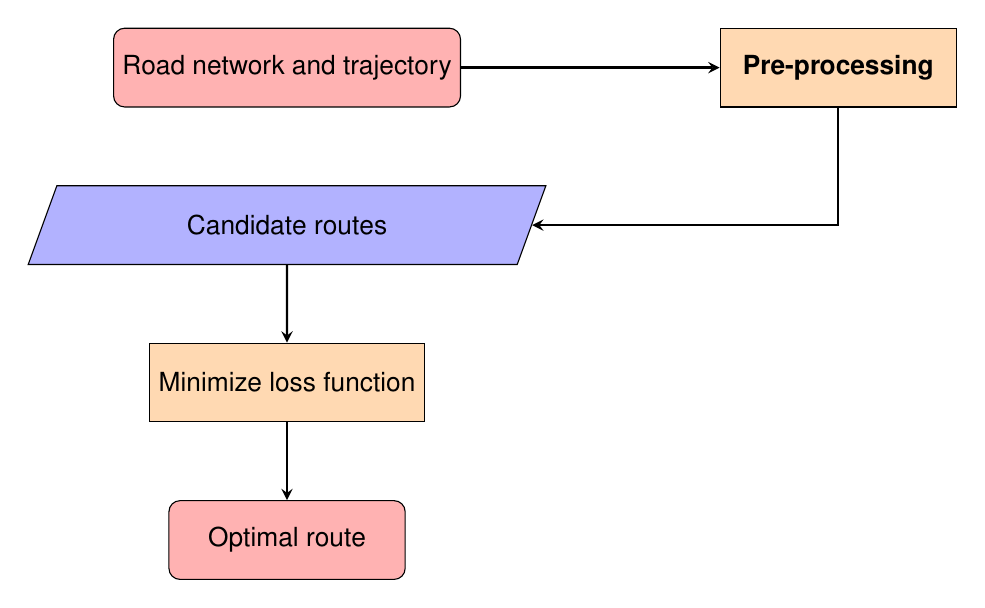
\begin{tikzpicture}[node distance=2cm]
\node (in1) [startstop] {Road network and trajectory};
\node (pre) [process, right of=in1, xshift=5cm] {\textbf{Pre-processing}};
%\node (pro1) [process, below of=in1] {Pre-processing};
\node (out1) [io, below of=in1] {Candidate routes};    
\node (pro2a) [process, below of=out1] {Minimize loss function };
\node (out2) [startstop, below of=pro2a] {Optimal route};


\draw [arrow] (in1) -- (pre);
\draw [arrow] (pre) |- (out1);
%\draw [arrow] (pro1) -- (out1);
\draw [arrow] (out1) -- (pro2a);
\draw [arrow] (pro2a) -- (out2);
\end{tikzpicture}}
\end{center}
\end{frame}

\begin{frame}{Sendai Map Revisited}

\ttfamily
Obtaining Candidate Routes (Dijsktra's Algorithm)\\
CPU times: user 45.8 s, sys: 49.7 ms, total: 45.9 s\\
Wall time: 45.9 s\\
\vspace{5mm}
Preprocessing Candidate Routes\\
CPU times: user 12.7 s, sys: 103 ms, total: 12.8 s\\
Wall time: 12.8 s

\end{frame}

\begin{frame}{Map-matching Pipeline}
\begin{center}
\scalebox{0.9}{
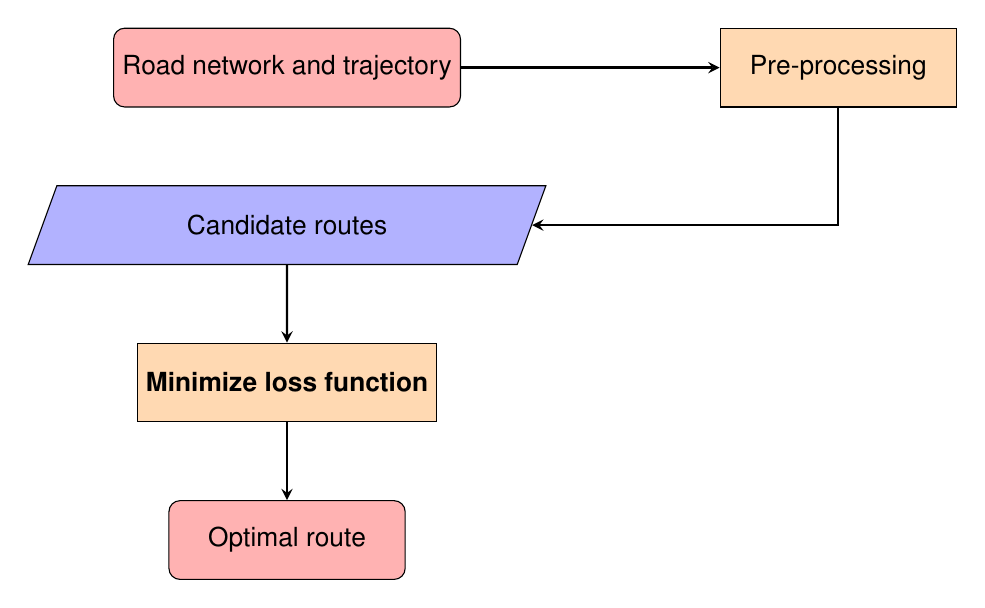
\begin{tikzpicture}[node distance=2cm]
\node (in1) [startstop] {Road network and trajectory};
\node (pre) [process, right of=in1, xshift=5cm] {Pre-processing};
%\node (pro1) [process, below of=in1] {Pre-processing};
\node (out1) [io, below of=in1] {Candidate routes};    
\node (pro2a) [process, below of=out1] {\textbf{Minimize loss function }};
\node (out2) [startstop, below of=pro2a] {Optimal route};


\draw [arrow] (in1) -- (pre);
\draw [arrow] (pre) |- (out1);
%\draw [arrow] (pro1) -- (out1);
\draw [arrow] (out1) -- (pro2a);
\draw [arrow] (pro2a) -- (out2);
\end{tikzpicture}}
\end{center}
\end{frame}


\begin{frame}{Sendai Map Revisited}
\ttfamily
Least Squares Runtime\\
CPU times: user 1.53 s, sys: 29.9 ms, total: 1.56 s\\
Wall time: 1.55 s\\
\vspace{5mm}
Inverse Squares Runtime\\
CPU times: user 14.2 s, sys: 392 ms, total: 14.6 s\\
Wall time: 10.2 s\\
\vspace{5mm}
Wasserstein Runtime\\
(Computation times vary wildly based on parameters-- anywhere from 20 seconds, to 20 minutes, to 2.5 hours)
  
\end{frame}

\begin{frame}{Sendai Map Revisited}
Unfortunately, due to FMM relying on outdated libraries, we could not produce an image demonstrating FMM's performance on the new trip data. Our preliminary findings demonstrated that FMM still performed poorly on the dataset. For the sake of comparison, recall FMM's results on the older GPS dataset:
\centering
\includegraphics[scale=0.21]{Jupyter Notebook LaTeX/oldfmmresults.png}\\

We also note that FMM runs in roughly 5 seconds on our current dataset.
\end{frame}

\begin{frame}{Sendai Map: Least Squares (Harmonic Oscillator) Result}
\centering
\includegraphics[scale=0.21]{Jupyter Notebook LaTeX/leastsquaressendai.png}
    
\end{frame}

\begin{frame}{Sendai Map: Inverse Squares (Electrical Method) Result}
\centering
\includegraphics[scale=0.21]{Jupyter Notebook LaTeX/electricsendai.png}
    
\end{frame}
\begin{frame}{Sendai Map: Wasserstein Method Result}
\centering
\includegraphics[scale=0.21]{Jupyter Notebook LaTeX/wassersteinsendai.png}
    
\end{frame}

\subsection{Computational Complexity}

\begin{frame}{Computational Complexity (Preprocessing)}
    
        \centering
    \includegraphics[scale=0.18]{Jupyter Notebook LaTeX/preprocessing.png}
    
    % \begin{table}[h]
    %     \centering
    %     \begin{tabular}{c||c|c|c|c}
    %     & n = 24 & n = 48 & n = 96 & n = 192 \\ \hline \hline \\
    %     k = 16 & 2min 56s & 2min 43s & 2min 33s & 2min 40s  \\
    %     k = 32 & 2min 36s & 2min 42s & 2min 55s & 4min 15s  \\
    %     k = 64 & 3min 14s & 3min 59s & 11min 45s & 28min 1s  \\
    %     k = 128 & 32min 26s & 37min 32s & 5h 20min 55s & 10hr 50m 50s  
    %     \end{tabular}
    %     \caption{Preprocessing times as a function of number of candidate routes (n) and (k-)nearest neighbors}
    %     \label{tab:preprocessing_times}
    % \end{table}
    
\end{frame}

\begin{frame}{Computational Complexity (Metric Calculations)}
%    While the accuracy of these methods are significantly improved over Fast Map Matching (Hidden Markov Model based), they come at the cost of high computation time.
    The following scatter plots demonstrates how computation grows as a function of input nodes.
\end{frame}

\begin{frame}{Computational Complexity (Metric Calculations)}
    \centering
    \includegraphics[scale=0.18]{Jupyter Notebook LaTeX/complexity1.png}
\end{frame}

\begin{frame}{Computational Complexity (Metric Calculations)}
    \centering
    \includegraphics[scale=0.18]{Jupyter Notebook LaTeX/complexity2.png}

\end{frame}

\begin{frame}{Computational Complexity}
    This suggests that simple distance methods (like inverse squares and least squares) have a computational complexity of $\mathcal{O}(n)$. Due to processing power, we could not obtain enough data to infer the computational complexity of the Wasserstein method. Because it relies on linear programming, we hypothesize that the growth rate is a polynomial of degree $>1$.\\
\vspace{5mm}
    Some aspects of these algorithms can be improved upon-- simple parallelization techniques offer a noticeable increase. However, other aspects are inherent to the method and are difficult to improve.
\end{frame}

\subsection{Preliminary Numerical Results}

\begin{frame}{Preliminary Numerical Results}
    Due to limits in processing power, we were unable to test our algorithms against all of the data in the dataset. 
    However, we demonstrate a few cases here.
\end{frame}

\begin{frame}{Preliminary Numerical Results}

\includegraphics[scale=0.35]{Jupyter Notebook LaTeX/fmmerror.png}
\includegraphics[scale=0.35]{Jupyter Notebook LaTeX/leastsquareerror.png}
\includegraphics[scale=0.35]{Jupyter Notebook LaTeX/electricerror.png}

\end{frame}



%%
% Jupyter Slides here: Sendai Notebook
%%
%\section{Conclusion and Future Work}
\subsection{Future Work}
\begin{frame}{Future Work (Implementation)}
    \begin{itemize}
        \item While a naive Dijkstra method generates a good set of candidate routes, it has many shortcomings. It is still relatively slow, it is conditional on the given parameters, and it cannot handle stranger routes (traversing an edge more than once). Each of these individually can be addressed; or it may be more suitable to find an alternative candidate route generation method.
        \item Investigate Wasserstein method inconsistencies more thoroughly
        \item Incomplete road networks
        \item Implement IMU-based map matching approaches
    \end{itemize}
\end{frame}


%%%%%%%%%%%%%%%%%%%%%%%%%%%%%%%%%%%%%%%%%%%%%%%%%%%%%
%%%%%%%%%%%%%%%%%%%%%%%%%%%%%%%%%%%%%%%%%%%%%%%%%%%%%
% \section{Implementation}
% \begin{frame}{Jupyter Demonstration}
% \centering
% \includegraphics[height=0.7\paperheight,keepaspectratio]{Jupyter Notebook LaTeX/output_3_0.png}

% \end{frame}

% \begin{frame}{Datasets}
    
% After formulating the proposed  mathematical methods into robust map-matching algorithms, we will implement them in python to evaluate their performance numerically using these datasets:
% \begin{itemize}
%     \item \textit{Dataset for testing and training of map-matching algorithms} \cite{KCMMN} (GPS only, has ground truths),
%     \item The BDD100K open data set provided by Berkeley \cite{yuBDD100KDiverseDriving2020} (for GPS and IMU data, no ground truths).\footnote{Because there are no public annotated ground truths, we compare our predictions with the standard EKF approach. This evaluation method is flawed but unavoidable.} % Describe what we used for ground truths
% \end{itemize}
% We will also compare the performance of our methods to a geometric method, such as point-to-curve, and HMM method, such as an extended Kalman filter (EKF) or Fast Map-Matching \cite{YG}.
    
% \end{frame}

% \begin{frame}{Evaluation}
%     How do we measure the accuracy of our prediction? 
    
%     \vspace{-2.5mm}
%     \begin{figure}[ht]
%     \centering
%     \def\svgwidth{\linewidth}
%     {\footnotesize
%     \input{error-formula.pdf_tex}}
%     \footnotesize
%     \begin{align*} 
% 	    d_0 &= \text{length of ground truth} \\
% 	    d_- &= \text{length of prediction route erroneously subtracted} \\
% 	    d_{+} &= \text{length of prediction route erroneously added}
%     \end{align*}
%     \normalsize
%     \caption{Error Formula by Newson and Krumm}
%     \label{fig:error-formula}
% \end{figure}
    
% \end{frame}

\begin{frame}
\frametitle{Thank You! And References}

\begin{thebibliography}{9}
\scriptsize{
% \bibitem{KB} Kolmogorov, A. N. and Barzdin, Ya. M.; On the realization of networks in three-dimensional space, in
% \textit{Selected Works of Kolmogorov}, Volume 3, ed. Shiryaev, A. N., Kluwer Academic Publishers, Dordrecht,
% 1993.


\bibitem[H]{H}  High-assurance Mobility Control Lab. \url{https://hmc.unist.ac.kr/research/autonomous-driving/}
\bibitem[KCMMN]{KCMMN} M. Kubi\u cka, A. Cela, P. Moulin, H. Mountier and S. I. Niculescu, \textit{Dataset for testing and training of map-matching algorithms}, In 2015 IEEE Intelligent Vehicles Symposium (IV), 1088--1093 (2015).
%\bibitem[LLY]{LLY} Y. Lin, L. Lu and S.-T. Yau, \textit{Ricci curvature of graphs}, Tohoku Math. J. (2) \textbf{63}(4) (2011), 605--627.
\bibitem[Sa]{Sa} F. Santambrogio, \textit{Optimal transport for applied mathematicians. Calculus of variations, PDEs, and modeling}, Progress in Nonlinear Differential Equations and their Applications, Birkh\"{a}user/Springer, Cham. (2015).
\bibitem[YCWXCLMD]{yuBDD100KDiverseDriving2020} F. Yu, H. Chen, X. Wang, W. Xian, Y. Chen, F. Liu, V. Madhavan and T. Darrell, \textit{BDD100K: A Diverse Driving Dataset for Heterogeneous Multitask Learning}, In Proceedings of the IEEE/CVF conference on computer vision and pattern recognition, 2636--2645 (2020).
\bibitem[YG]{YG} C. Yang and G. Gid\' ofalvi, \textit{Fast map matching, an algorithm for integrating a hidden Markov model with precomputation}, International Journal of Geographical Information Science. Taylor \& Francis, \textbf{32}(3), 547--570 (2018).}
\end{thebibliography}

\end{frame}

\end{document}
